\section{Results}\label{sec:Charmonia_Results}

This section presents the measurements of the charmonium production in \RunPbPb and \Runpp collisions at $\sqrtsnn = \SI{5.02}{\TeV}$. The results of the nonprompt fraction of \JPsi mesons are shown in \sect{sec:Charmonia_Results_BFrac_JPsi}. In \sect{sec:Charmonia_Results_XSec_JPsi}, the measurements of the normalised cross sections of \JPsi-meson production in \Runpp and \RunPbPb collisions, are reported. The nuclear modification factor of \JPsi mesons and the double ratio of prompt \PsiP over \JPsi meson yields are presented in \sect{sec:Charmonia_Results_RAA_JPsi} and \sect{sec:Charmonia_Results_DoubleRatio}, respectively.

\subsection{Nonprompt fraction of \texorpdfstring{\JPsi}{J/psi} mesons}\label{sec:Charmonia_Results_BFrac_JPsi}

The fraction of \JPsi mesons coming from b-hadron decays is measured in \Runpp and \RunPbPb collisions at $\sqrtsnn = \SI{5.02}{\TeV}$, for different dimuon rapidity and \pt intervals. The nonprompt \JPsi-meson  fraction is extracted by performing 2D fits to the \mMuMu and \ctau distributions in data. The extracted fractions are corrected for detector acceptance and efficiency, in each analysis bin and collision system, according to:

\begin{equation}
 \bJPsi = \bJPsi^{\text{raw}} \left( \frac{\left(\accJPsi\times\effJPsi\right)^{\text{P}}}{\bJPsi^{\text{raw}}\left(\accJPsi\times\effJPsi\right)^{\text{P}} + \left(1-\bJPsi^{\text{raw}}\right)\left(\accJPsi\times\effJPsi\right)^{\text{NP}}} \right)
 \label{eq:BFracCorr}
\end{equation}

where $\bJPsi^{\text{raw}}$ is the nonpromt \JPsi-meson fraction determined from the data fits, and $(\accJPsi\times\effJPsi)^{\text{P}}$ and $(\accJPsi\times\effJPsi)^{\text{NP}}$ are the acceptance times efficiency factors for prompt and nonprompt \JPsi mesons, respectively. The systematic uncertainty of the acceptance and efficiency corrections, and the statistical uncertainty from the 2D fits, are propagated to the measured nonprompt \JPsi-meson fraction. 

\fig{fig:bFracspp} shows the \bJPsi results as a function of dimuon \pt and rapidity, measured in \Runpp and \RunPbPb collisions. The nonprompt fraction of \JPsi mesons is observed to not vary significantly with respect to rapidity. However, it depends strongly on \ptMuMu, increasing from $\sim{0.2}$ at $\ptMuMu \approx 6.5$~\GeVc to $\sim{0.6}$ at $\ptMuMu > 30$~\GeVc. The \bJPsi measurements are also seen to be slightly larger in \RunPbPb compared to \Runpp collisions at $\ptMuMu < 20$~\GeVc. Considering the significant \bJPsi fraction measured at high \pt, these results reaffirm the need to distinguish the  contributions from prompt and nonprompt \JPsi mesons, in order to disentangle the hot nuclear matter effects that impact the production of charmonia and b hadrons.

\begin{figure}[hbtp]
 \centering
  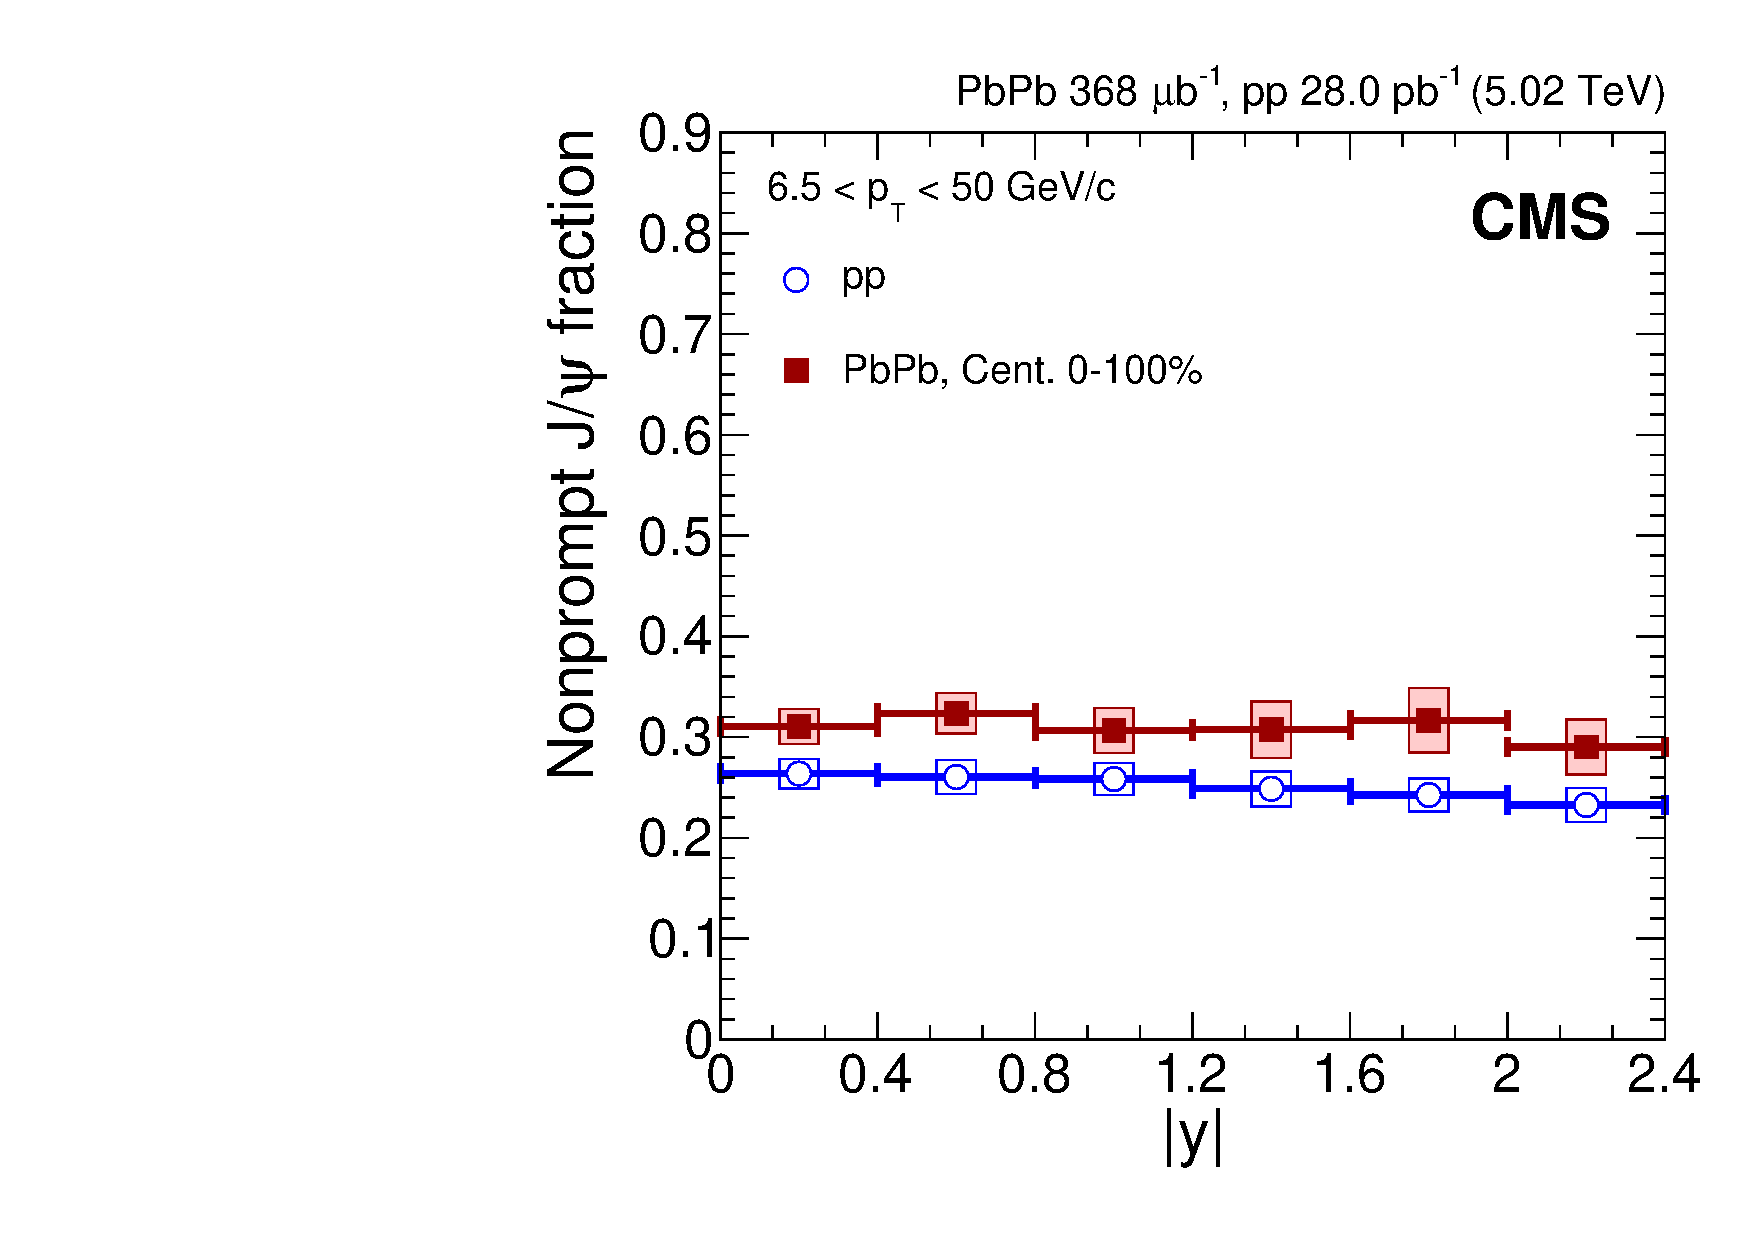
\includegraphics[width=0.45\textwidth]{Figures/Charmonia/Results/JPsi_BFraction/Figure_002-b.pdf}
  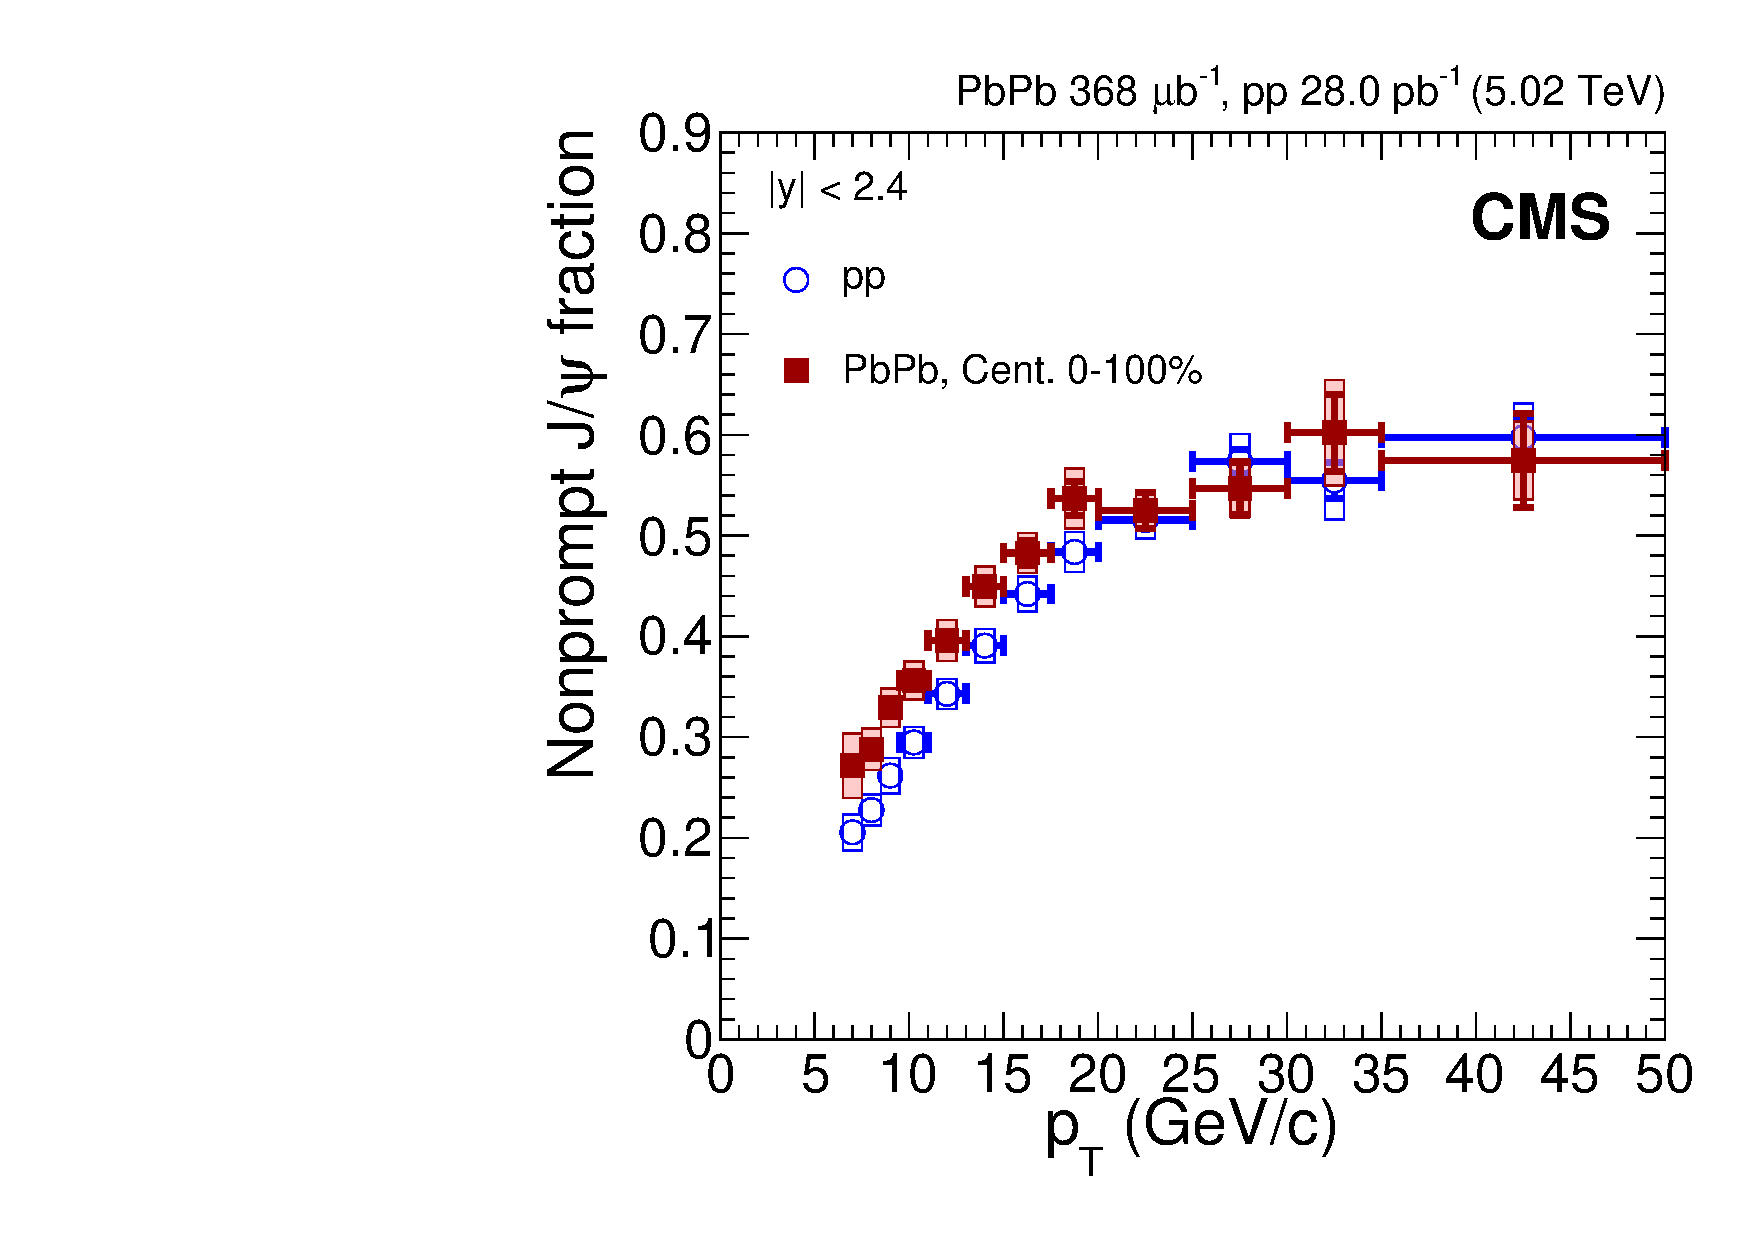
\includegraphics[width=0.45\textwidth]{Figures/Charmonia/Results/JPsi_BFraction/Figure_002-a.pdf}
 \caption{Nonprompt fraction of \JPsi mesons measured in \Runpp and \RunPbPb collisions, as a function of dimuon rapidity (left) and \pt (right). The boxes (bars) represent the systematic (statistical) uncertainties. Figures published in Ref.~\cite{CMS_JPsi_PbPb_5p02TeV}.}
 \label{fig:bFracspp}
\end{figure}

\subsection{Cross section of prompt and nonprompt \texorpdfstring{\JPsi}{J/psi} mesons}\label{sec:Charmonia_Results_XSec_JPsi}

The \JPsi-meson production cross sections are derived from the measured number of prompt and nonprompt \JPsi mesons as:

\begin{equation}
 \nJPsi = \frac{\nJPsi^{\text{raw}}}{\left(\accJPsi\times\effJPsi\right)}
 \label{eq:NCorr}
\end{equation}

where $\nJPsi^{\text{raw}}$ is the number of prompt or nonprompt \JPsi mesons extracted from the 2D fits to the \mMuMu and \ctau distributions in data, and $\effJPsi$ and $\accJPsi$ are the corresponding \JPsi-meson efficiency and acceptance, respectively. In the case of \Runpp collisions, the production cross section of prompt and nonprompt \JPsi mesons decaying into \mumu is computed as follows:

\begin{equation}
 B\left(\JPsiToMuMu\right) \frac{\ddd{\sigma}_{\JPsi}^{\pp}}{\dd{\ptMuMu}\dd{\rapMuMu}} = \frac{1}{\Lumi_{\pp}}\left(\frac{\nJPsi^{\pp}}{\Delta{\ptMuMu}\Delta{\rapMuMu}}\right)
 \label{eq:XSec_PP}
\end{equation}

where $B$ represents the branching ratio of \JPsiToMuMu decays, $\nJPsi^{\pp}$ is the number of prompt or nonprompt \JPsi mesons measured in \Runpp collisions, $\Lumi_{\pp} = 28.0{\pm}0.6$~\pbinv is the recorded integrated luminosity of the \Runpp data sample, and $\Delta{\ptMuMu}$ and $\Delta{\rapMuMu}$ are the widths of the dimuon \pt and rapidity intervals in which the measurement is performed.

In order to directly compare the \RunPbPb measurements with those from \Runpp collisions, the \JPsiToMuMu cross section in \RunPbPb collisions is presented in the following way:

\begin{equation}
 B\left(\JPsiToMuMu\right) \frac{\ddd{\sigma}_{\JPsi}^{\PbPb}}{\dd{\ptMuMu}\dd{\rapMuMu}} = \frac{1}{\avgtaa\cdot\nMB}\left(\frac{\nJPsi^{\pp}}{\Delta{\ptMuMu}\Delta{\rapMuMu}}\right)
 \label{eq:XSec_PbPb}
\end{equation}

where $\nMB = (2.37{\pm}0.05)\times{10^{9}}$ represents the efficiency-corrected number of minimum bias events sampled by the analysis trigger and $\avgtaa = 5.61^{+0.16}_{-0.19}$ is the nuclear-overlap function integrated over the $0-100\%$ centrality range. The centrality-integrated \taa is equal to $\text{A}^{2}/\sigma^{\text{inel}}_{\PbPb}$, where $\text{A} = 208$ is the atomic number of Pb ions and $\sigma^{\text{inel}}_{\PbPb} = \nMB/\Lumi_{\PbPb}$ is the total \PbPb inelastic cross section.

The systematic uncertainties that impacts the measurement of the prompt and nonprompt \JPsiToMuMu cross sections in \Runpp and \RunPbPb collisions are:
\begin{itemize}
 \item The uncertainty on the \JPsi-meson extraction. It is associated to the parametrisation of the dimuon \mMuMu and \ctau distributions, and it is determined by varying the different components of the 2D fit model as described in Sections \ref{sec:Charmonia_Analysis_JPsiYieldSystematics_InvMass} and \ref{sec:Charmonia_Analysis_JPsiYieldSystematics_Ctau}.
 \item The uncertainty on the efficiency estimation. It includes the uncertainties due to the \tnp corrections applied to the efficiency, the \JPsi-meson \pt and rapidity weighing applied to the simulated dimuons, and the statistics of the simulated samples, as detailed in \sect{sec:Charmonia_Analysis_JPsiYieldSystematics_Efficiency}.
 \item The uncertainty on the measurement of the number of minimum bias events \nMB probed by the dimuon trigger, which corresponds to 2\%.
 \item The uncertainty on the \Runpp integrated luminosity. It has been derived by the CMS collaboration and corresponds to 2.3\%~\cite{LUMI_pp_5p02TeV}.
 \item The uncertainty on the \avgtaa computation. The \avgtaa relative asymmetric uncertainty in the centrality range $0-100\%$ is [$-3.4\%$,$+2.8\%$].
\end{itemize}

The global uncertainties (i.e. the same across all measurements) of the \JPsi-meson cross sections correspond to: the \Runpp integrated luminosity uncertainty of 2.3\% for \Runpp collisions, and the \avgtaa and \nMB uncertainties, which quadrature sums to a relative asymmetric uncertainty of [$-3.9\%$,$+3.4\%$], for \RunPbPb collisions.

The results of the \JPsi-meson cross sections, measured in \Runpp and \RunPbPb collisions are presented in \fig{fig:Jpsi_XSec}. The \JPsi-meson cross sections decrease rapidly towards higher \ptMuMu values, with the same trend between prompt and nonprompt \JPsi mesons, and between both collisions systems. The measurements as a function of rapidity are seen to decrease when approaching the forward region ($|\rapMuMu| > 1.2$), and similar trends are also observed between the different measurements.

\begin{figure}[htb!]
 \centering
  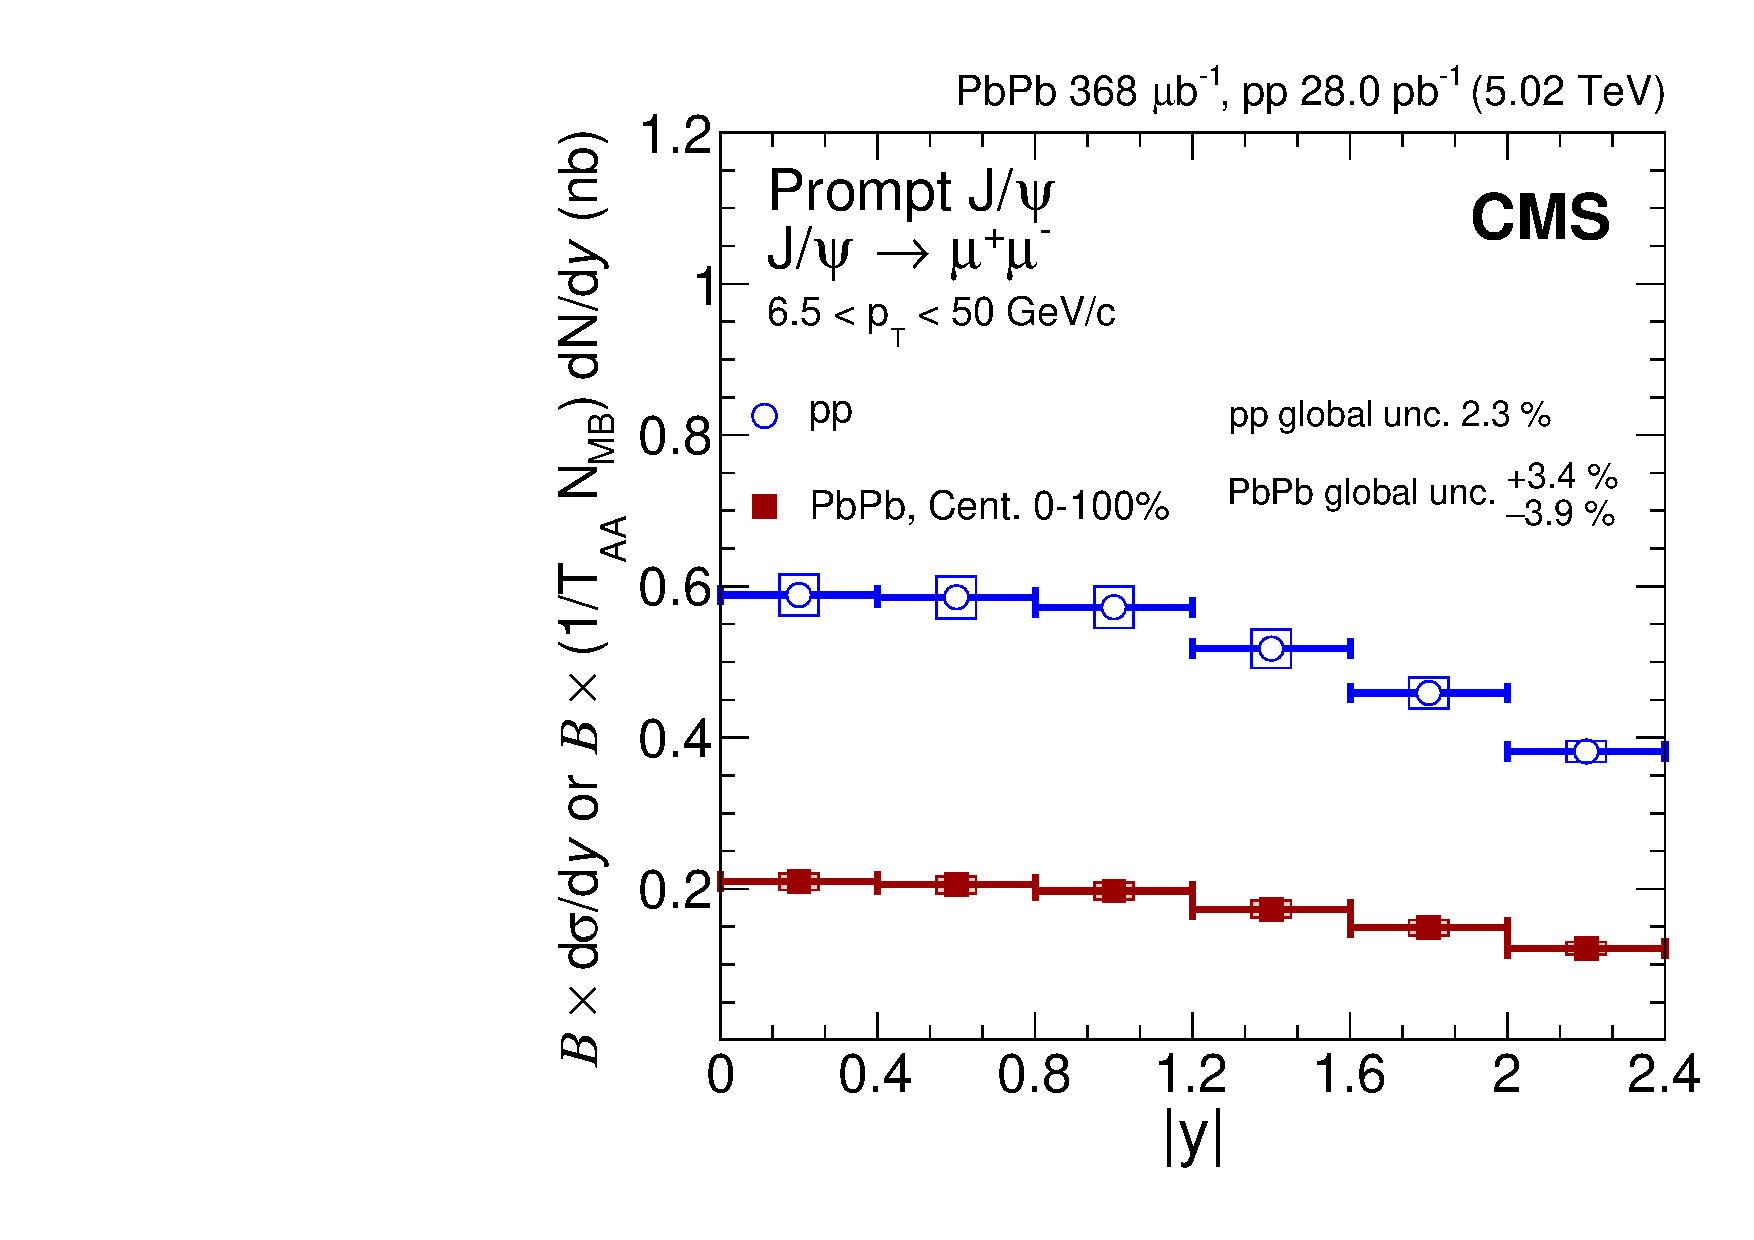
\includegraphics[width=0.45\textwidth]{Figures/Charmonia/Results/Prompt_JPsi_XSec/Figure_003-c.pdf}
  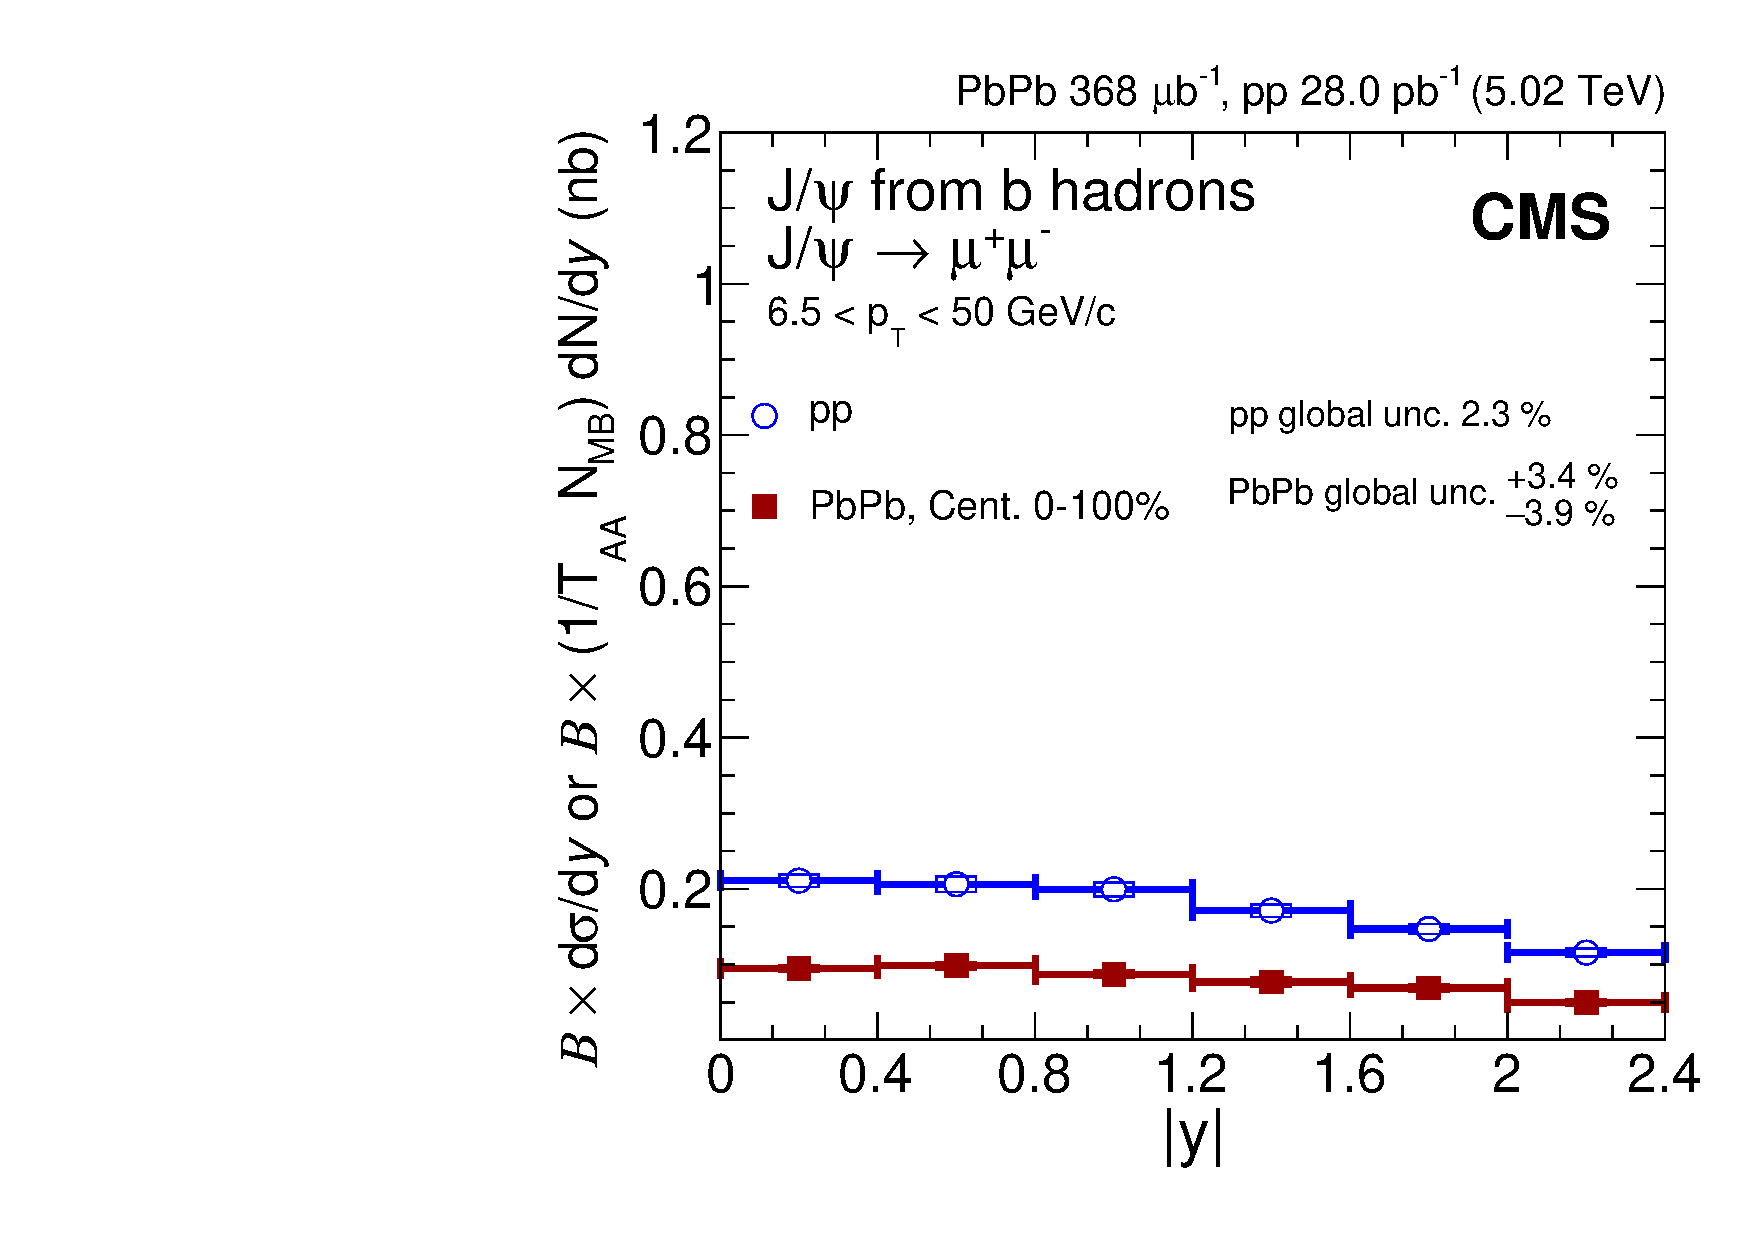
\includegraphics[width=0.45\textwidth]{Figures/Charmonia/Results/NonPrompt_JPsi_XSec/Figure_003-d.pdf}\\
  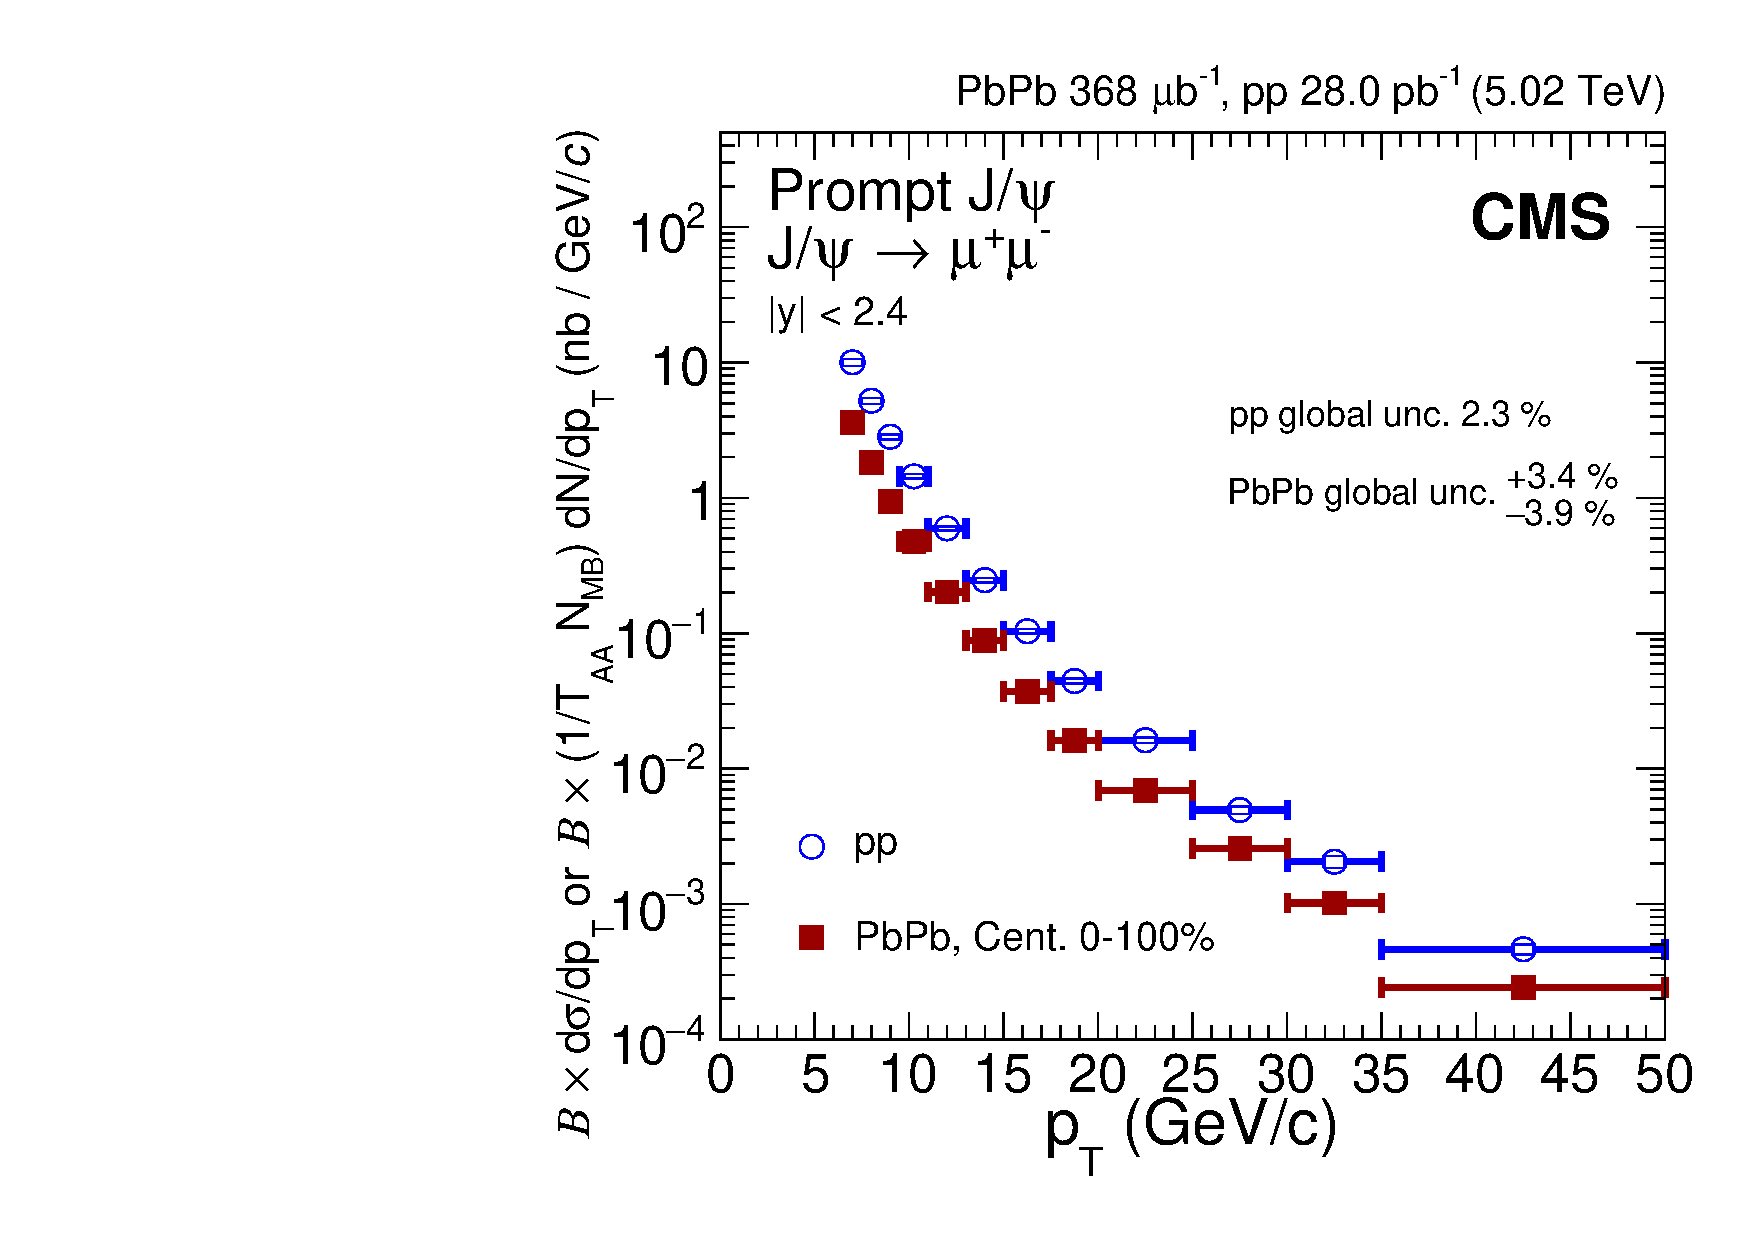
\includegraphics[width=0.45\textwidth]{Figures/Charmonia/Results/Prompt_JPsi_XSec/Figure_003-a.pdf}
  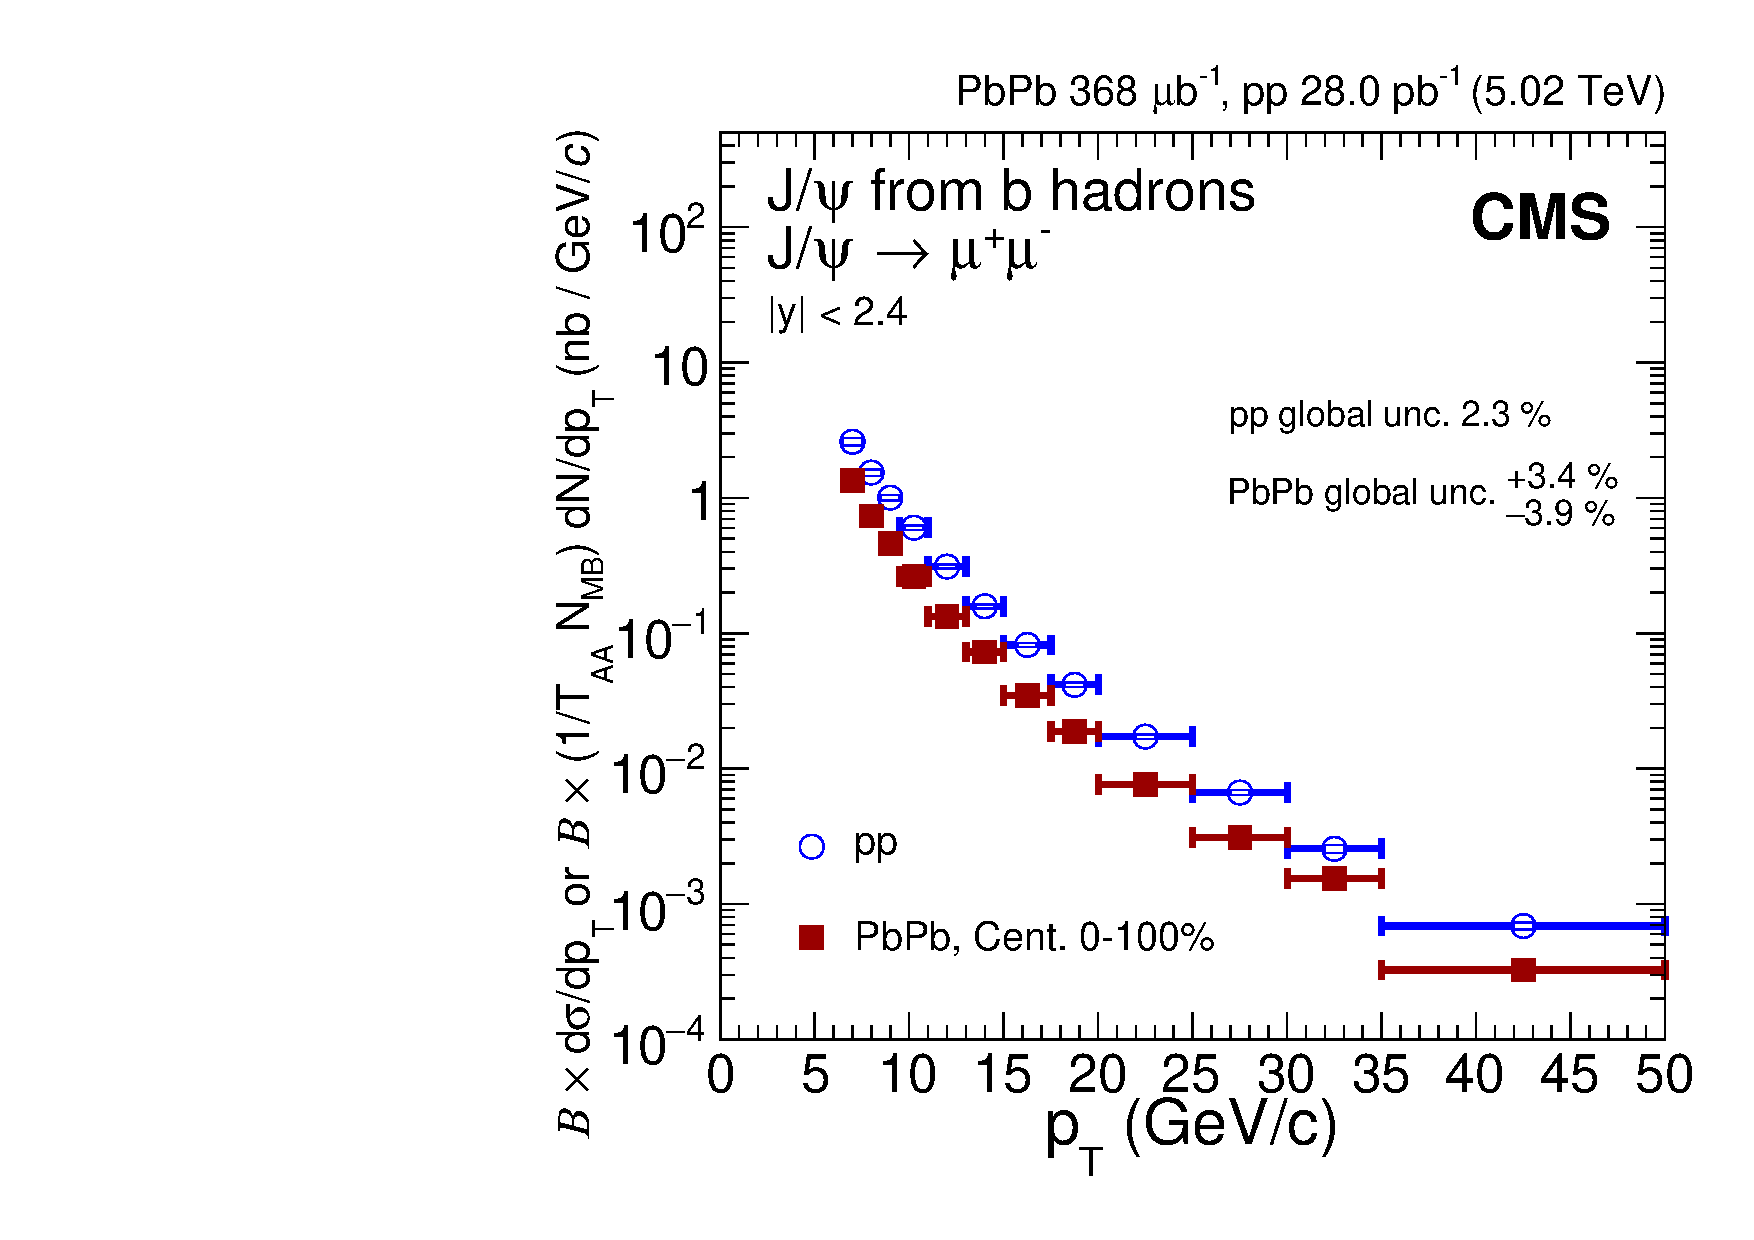
\includegraphics[width=0.45\textwidth]{Figures/Charmonia/Results/NonPrompt_JPsi_XSec/Figure_003-b.pdf}
  \caption{Differential cross section of the production of prompt (left) and nonprompt (right) \JPsi mesons decaying into \mumu, as a function of dimuon rapidity (top) and \pt (bottom) in \Runpp (blue open circles) and \RunPbPb (red squares) collisions. The boxes (bars) represent the systematic (statistical) uncertainties. The global relative uncertainties are written in the plots. Figures published in Ref.~\cite{CMS_JPsi_PbPb_5p02TeV}.}
 \label{fig:Jpsi_XSec}
\end{figure}

\subsection{Nuclear modification factor of \texorpdfstring{\JPsi}{J/psi} mesons}\label{sec:Charmonia_Results_RAA_JPsi}

The modification of the prompt and nonprompt production of \JPsi mesons in \RunPbPb collisions is studied  by measuring the nuclear modification factor, computed from the ratio of \PbPb-to-\pp cross sections presented in the previous section. The nuclear modification factor of \JPsi mesons is defined as:

\begin{equation}
 \raa^{\JPsi} = \left(\frac{{\ddd{\sigma}_{\JPsi}^{\PbPb}}\biggr/{\dd{\ptMuMu}\dd{\rapMuMu}}}{{\ddd{\sigma}_{\JPsi}^{\pp}}\biggr/{\dd{\ptMuMu}\dd{\rapMuMu}}}\right) = \frac{\Lumi_{pp}}{\avgtaa\cdot\nMB\cdot\Delta{\text{cent}}}\left(\frac{\nJPsi^{\PbPb}}{\nJPsi^{\pp}}\right)
 \label{eq:RAA}
\end{equation}

where $\Delta{\text{cent}}$ is the fraction of the total hadronic inelastic cross section sampled in the measured centrality range (e.g. 0.3 for 70--100\%). The measurements of the \JPsi-meson nuclear modification factor are performed as a function of the dimuon \pt, rapidity and the average number of participants \avgnpart.

The global uncertainties that enters in the measurement of the nuclear modification factor depends on which variable is used to bin the data. On the one hand, if the results are measured differentially in centrality, the global uncertainties include the statistical and systematic uncertainty of the \JPsi-meson cross section in \Runpp collisions, and the \nMB uncertainty of the \RunPbPb data. On the other hand, if the measurements are performed in different \ptMuMu or \rapMuMu intervals, then the global uncertainty includes the \Runpp integrated luminosity uncertainty, the \RunPbPb \nMB uncertainty and the uncertainty on the \avgtaa corresponding to the centrality range probed. The \avgtaa uncertainties are found to vary from 2\% in central \RunPbPb collisions to 16\% in the most peripheral ones, as presented in \tab{tab:TAAValues}.


\subsubsection{Prompt \texorpdfstring{\JPsi}{J/psi}-meson \texorpdfstring{\raa}{RAA}}\label{sec:Charmonia_Results_RAA_JPsi_Prompt}

The \raa results as a function of \ptMuMu, rapidity and \avgnpart are shown in \fig{fig:PromptJpsi_ComparisonWith2p76_RAA}. The measurements are compared with the CMS results derived at $\sqrtsnn = \SI{2.76}{\TeV}$ and found to be in agreement within uncertainties.

\begin{figure}[htb!]
  \centering
    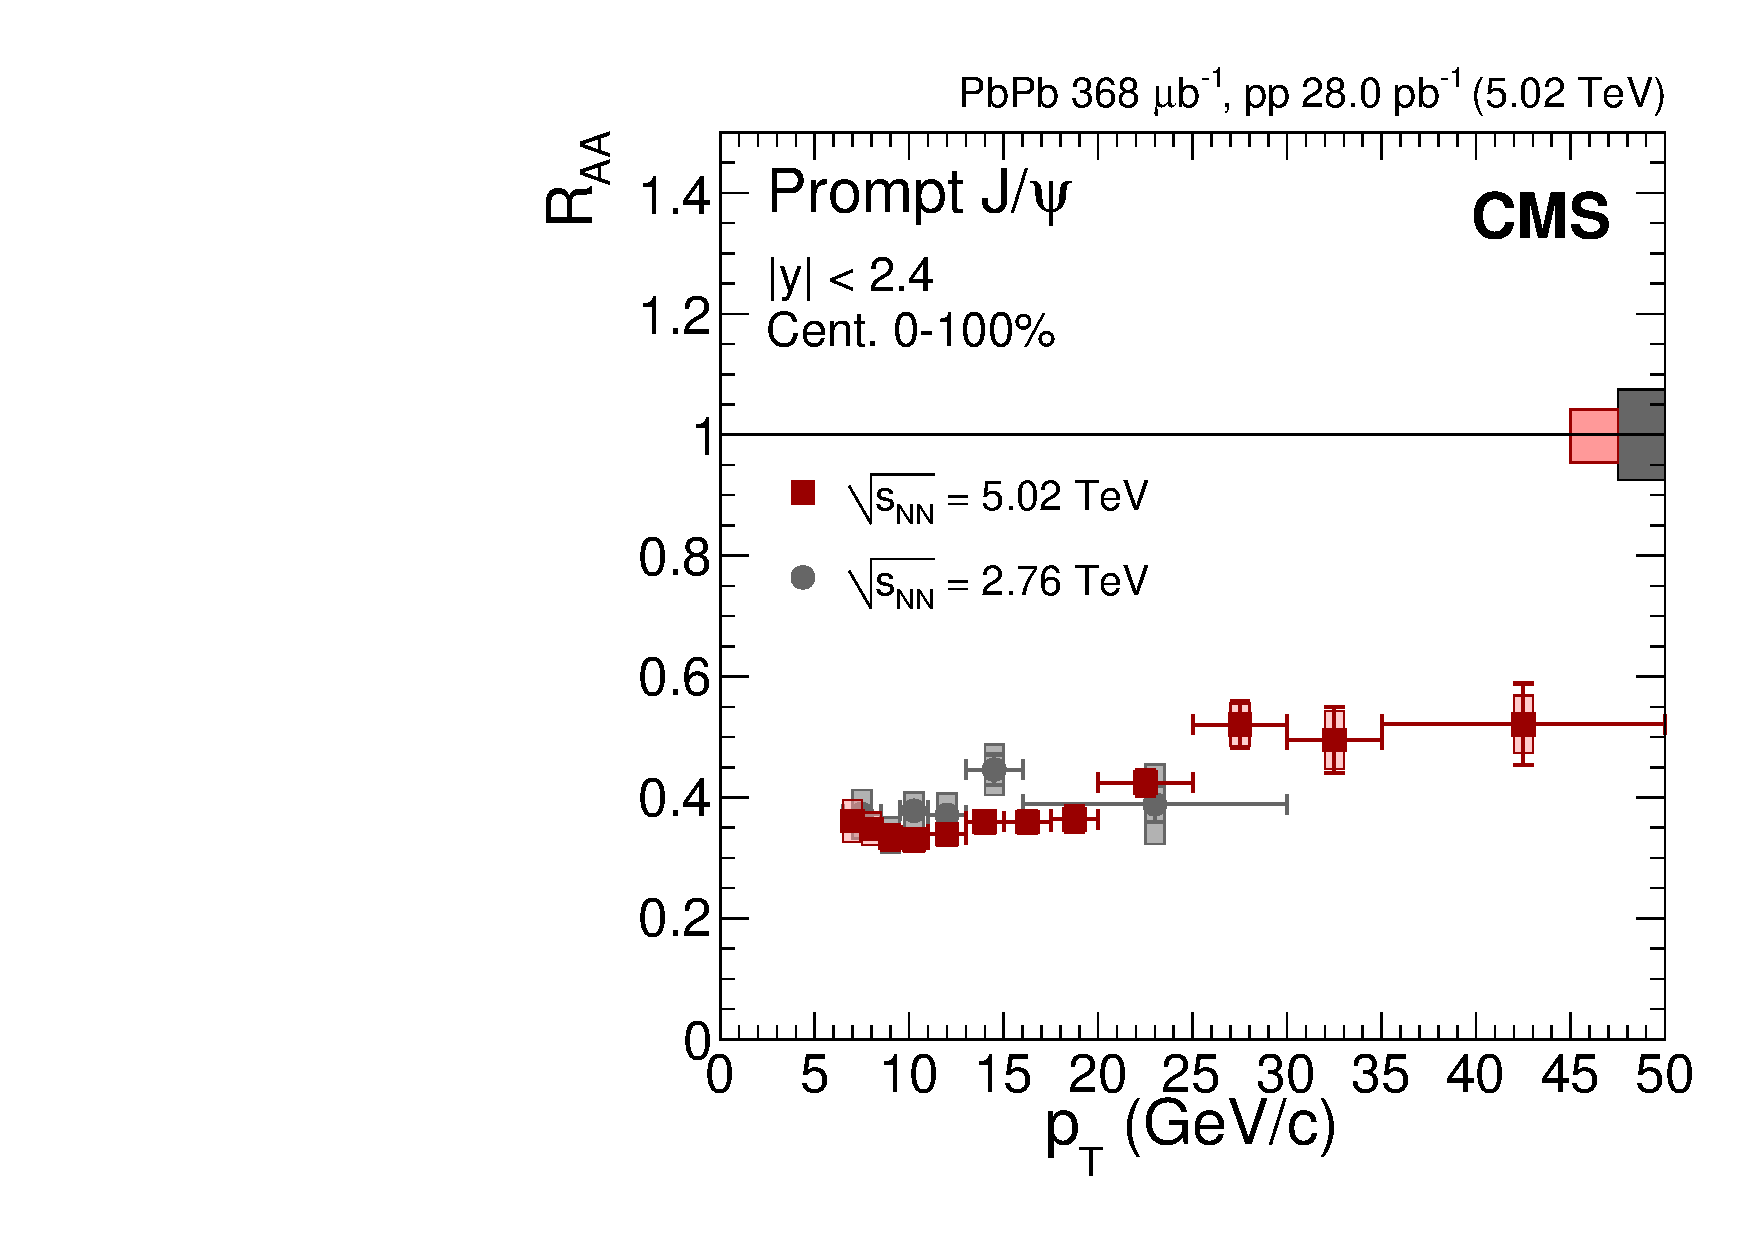
\includegraphics[width=0.32\textwidth]{Figures/Charmonia/Results/ComparisonWith2p76TeV/Prompt_JPsi_RAA/Figure_004-c.pdf}
    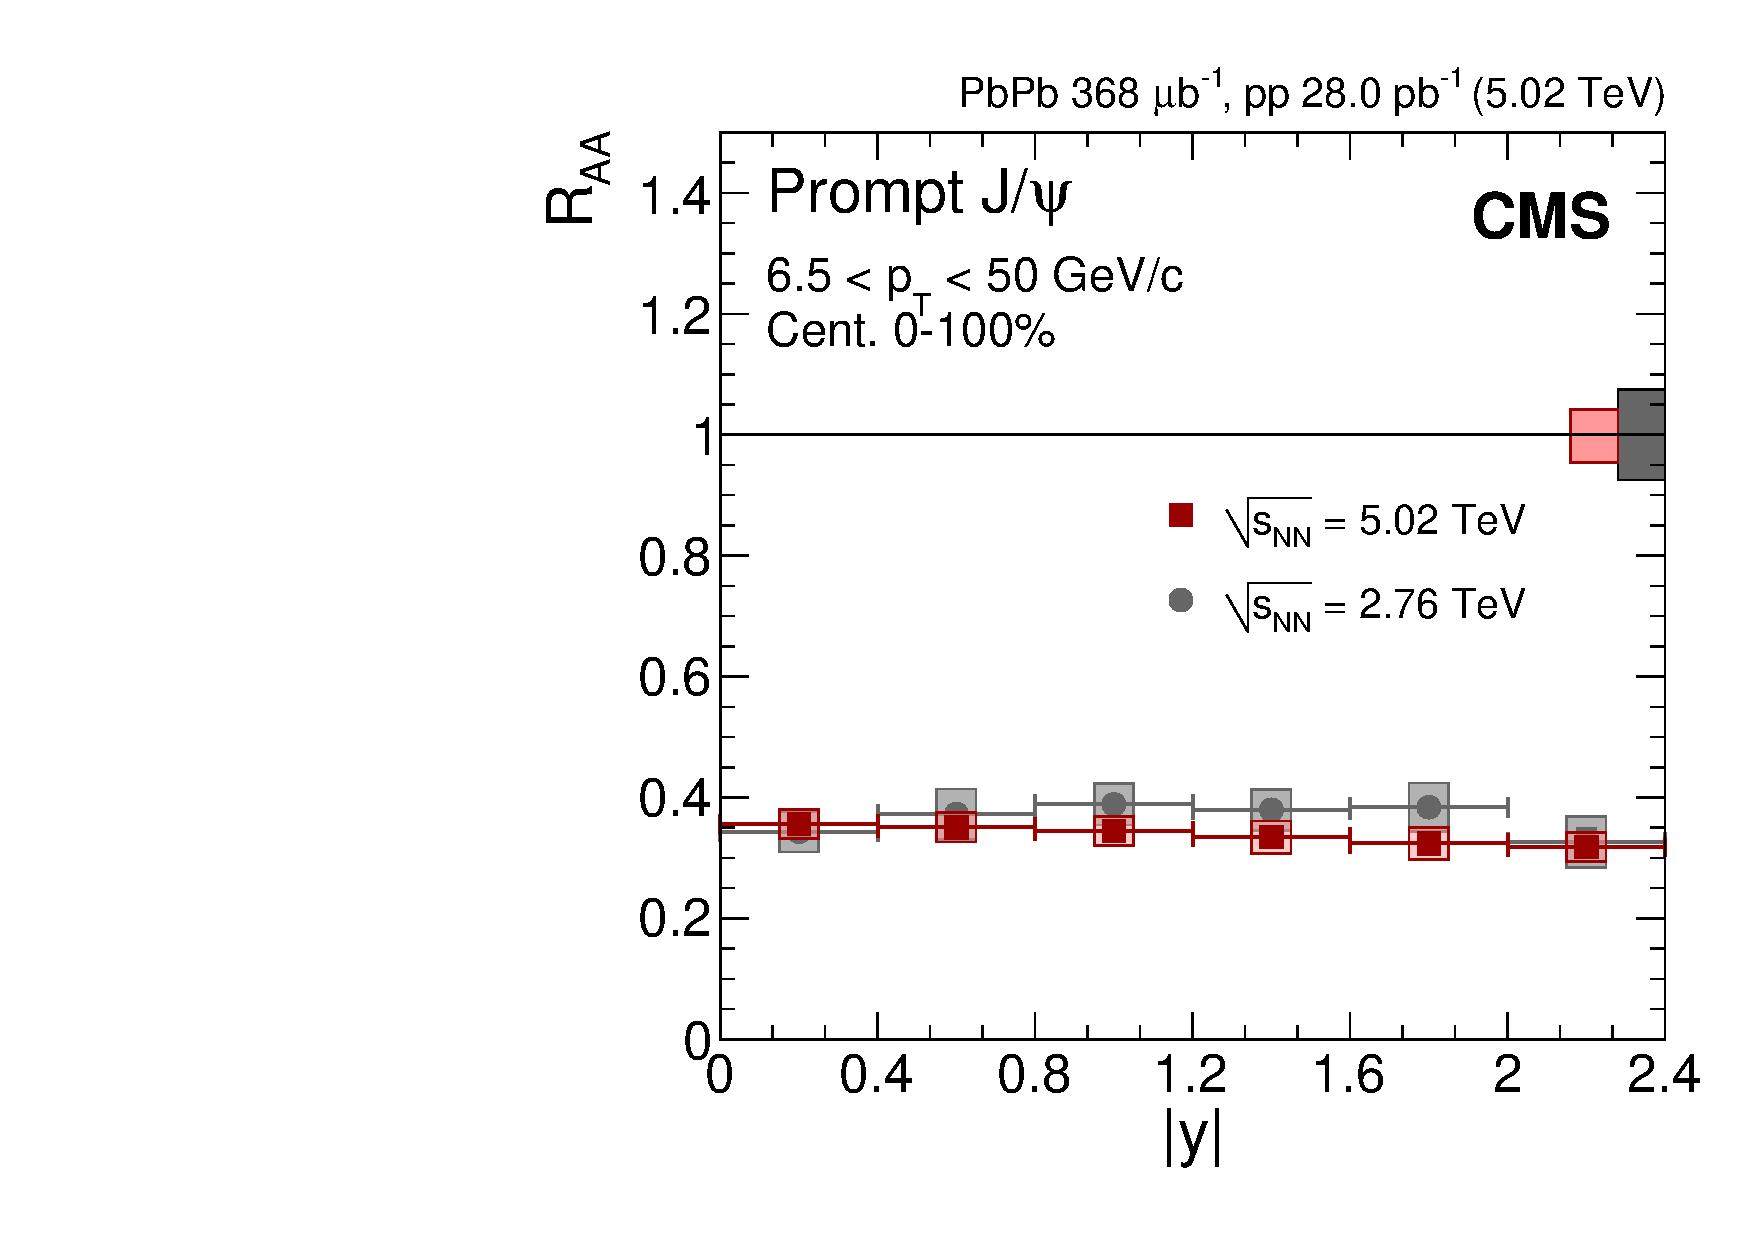
\includegraphics[width=0.32\textwidth]{Figures/Charmonia/Results/ComparisonWith2p76TeV/Prompt_JPsi_RAA/Figure_004-a.pdf}
    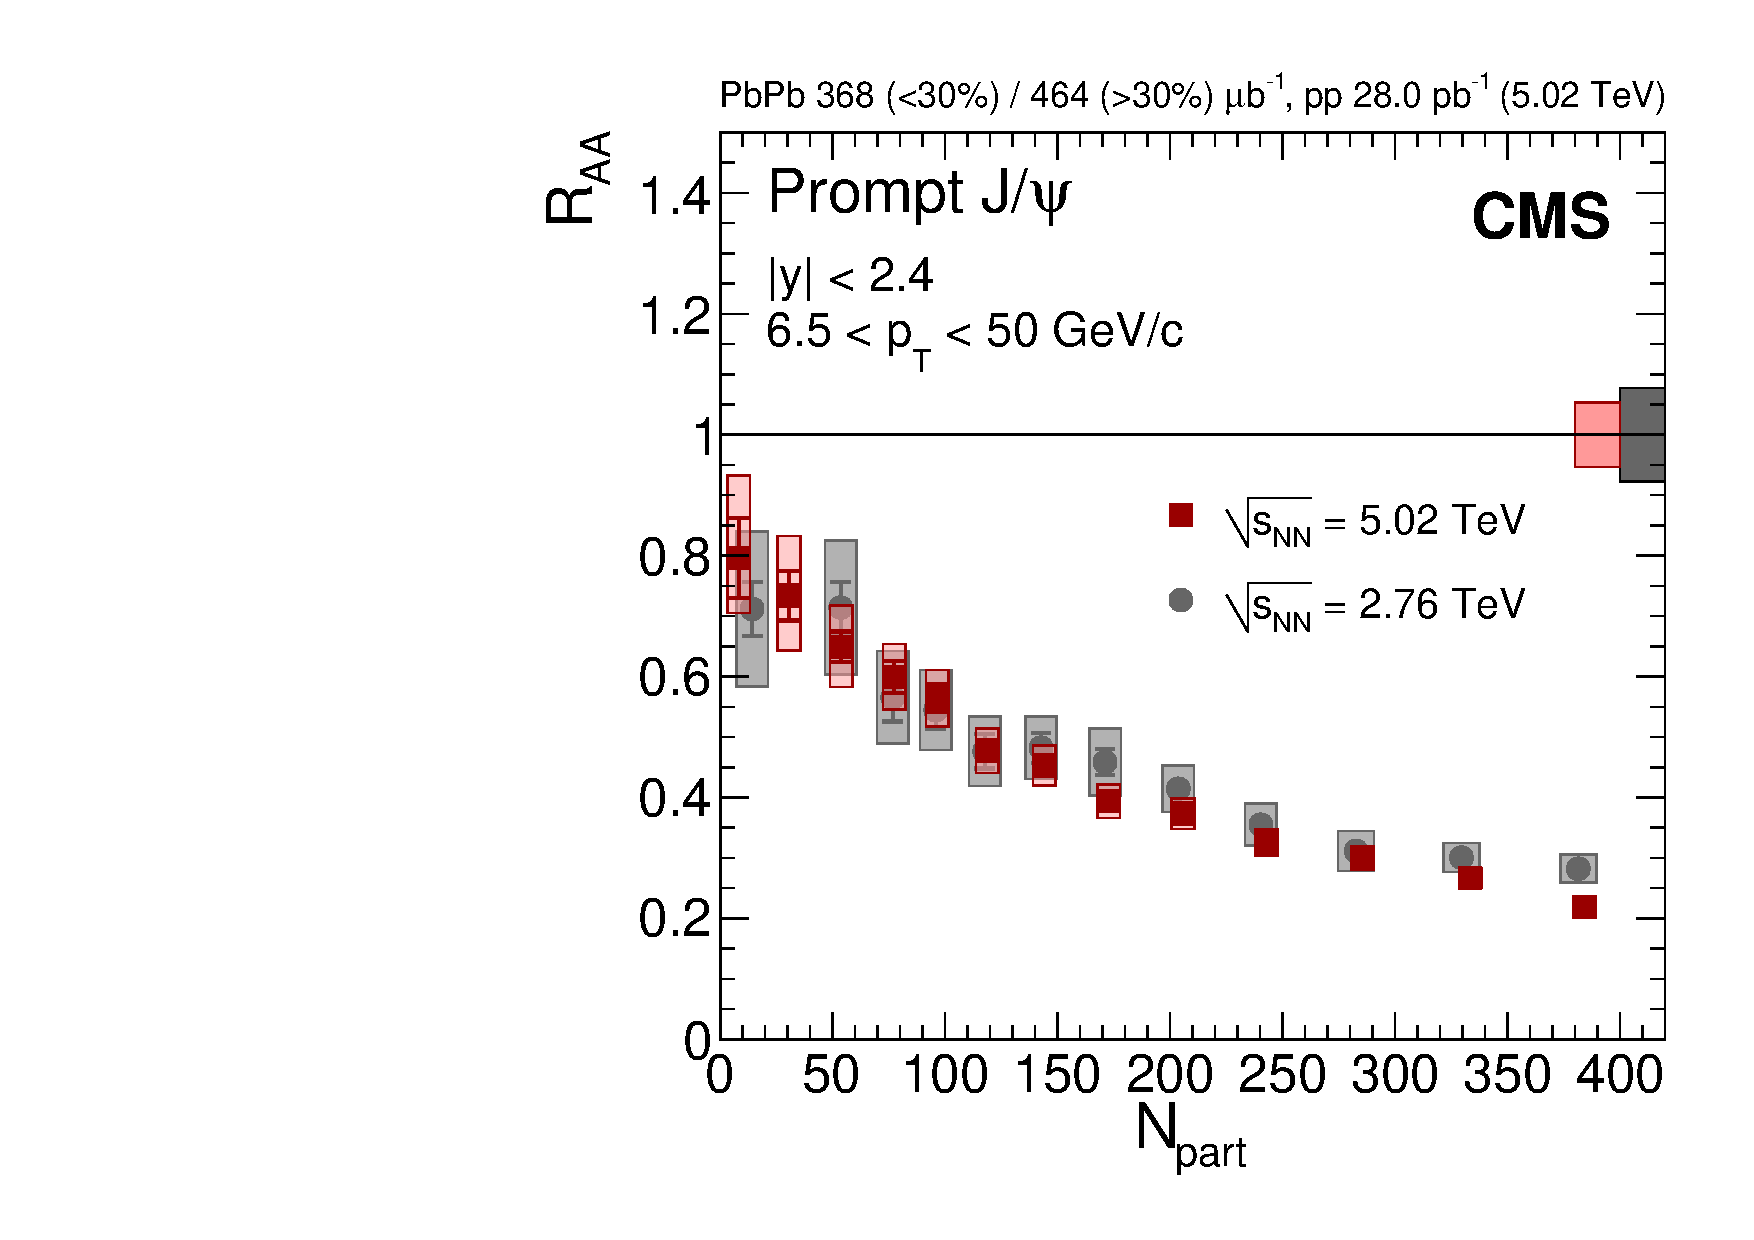
\includegraphics[width=0.32\textwidth]{Figures/Charmonia/Results/ComparisonWith2p76TeV/Prompt_JPsi_RAA/Figure_004-b.pdf}
    \caption{Nuclear modification factor of prompt \JPsi mesons measured at $\sqrtsnn = \SI{2.76}{\TeV}$~\cite{CMS_JPsi_PbPb_2p76TeV} (grey circles) and $\sqrtsnn = \SI{5.02}{\TeV}$~\cite{CMS_JPsi_PbPb_5p02TeV} (red squares), as a function of dimuon \pt (left), rapidity (middle) and \avgnpart (right). The boxes (bars) represent the systematic (statistical) uncertainties. The size of the global relative uncertainties are depicted in the boxes plotted at $\raa=1$. Figures published in Ref.~\cite{CMS_JPsi_PbPb_5p02TeV}.}
    \label{fig:PromptJpsi_ComparisonWith2p76_RAA}
\end{figure}

The prompt \JPsi-meson \raa is less than unity in all measurements, which means that prompt \JPsi mesons are suppressed in \RunPbPb collisions. It is observed that the dependence on \ptMuMu is mostly flat at $\ptMuMu > 6.5$~GeVc, except in the highest \pt intervals ($\ptMuMu > 25$~\GeVc), where the prompt \JPsi-meson suppression is seen to be weaker. Moreover, the prompt \JPsi mesons are more suppressed toward central collisions, which is consistent with the picture of colour-screening due to the QGP.

Double-differential results as a function of \ptMuMu and \avgnpart are displayed in \fig{fig:PromptJpsi_RAA}. The \ptMuMu dependence is presented for the mid- ($|\rapMuMu| < 0.6$) and most forward ($2.0 < |\rapMuMu| < 2.4$) rapidity regions, while the measurements as a function of \avgnpart are shown in two dimuon \pt intervals: $3 < \ptMuMu < 6.5$~\GeVc and $6.5 < \ptMuMu < 50$~\GeVc, at forward rapidity. An indication of less suppression is seen in central collisions ($\avgnpart > 200$, corresponding to 0-30\% centrality) for lower \ptMuMu values ($3.0 < \ptMuMu < 6.5$~\GeVc). Such reduction in the \JPsi-meson suppression could be caused by possible contributions from regenerated charmonia due to the hot medium.

\begin{figure}[htb!]
 \centering
  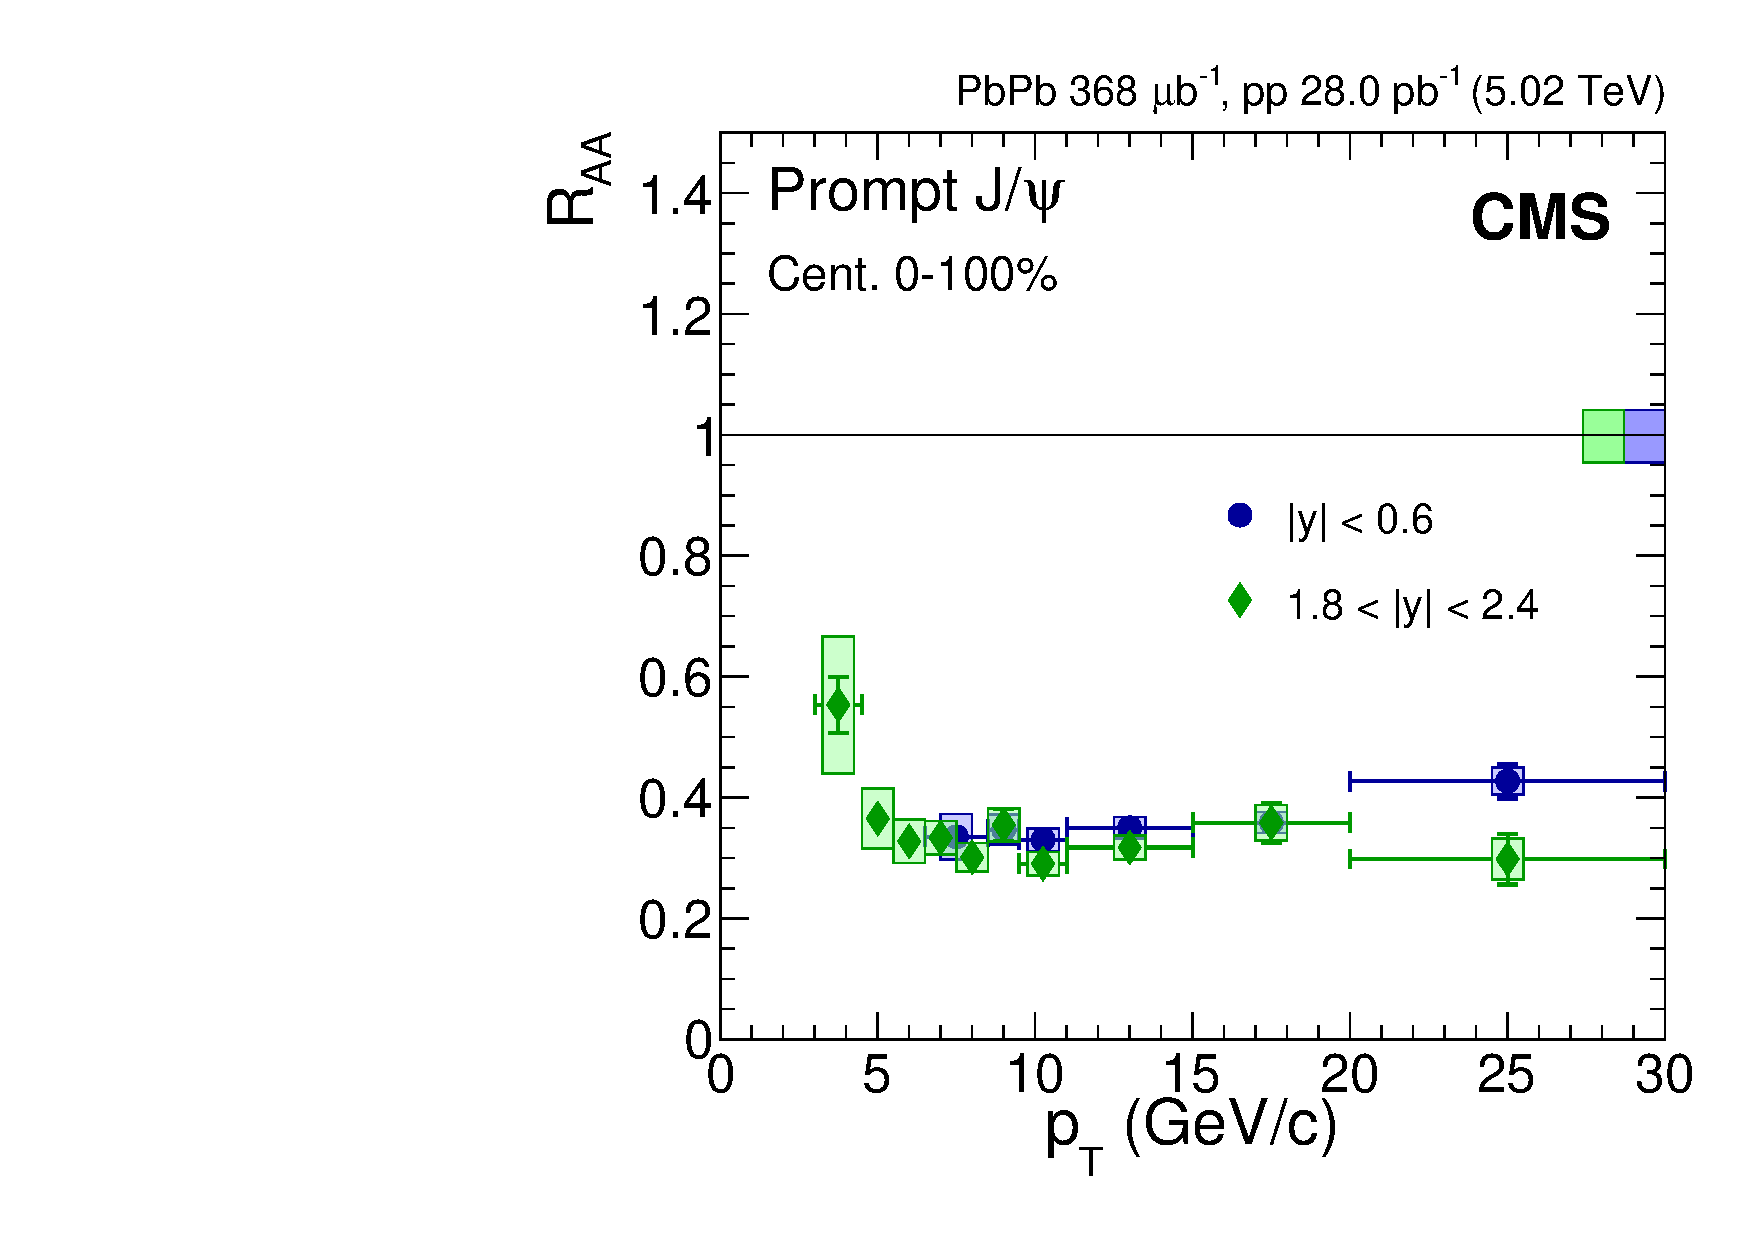
\includegraphics[width=0.45\textwidth]{Figures/Charmonia/Results/Prompt_JPsi_RAA/Figure_005-a.pdf}
  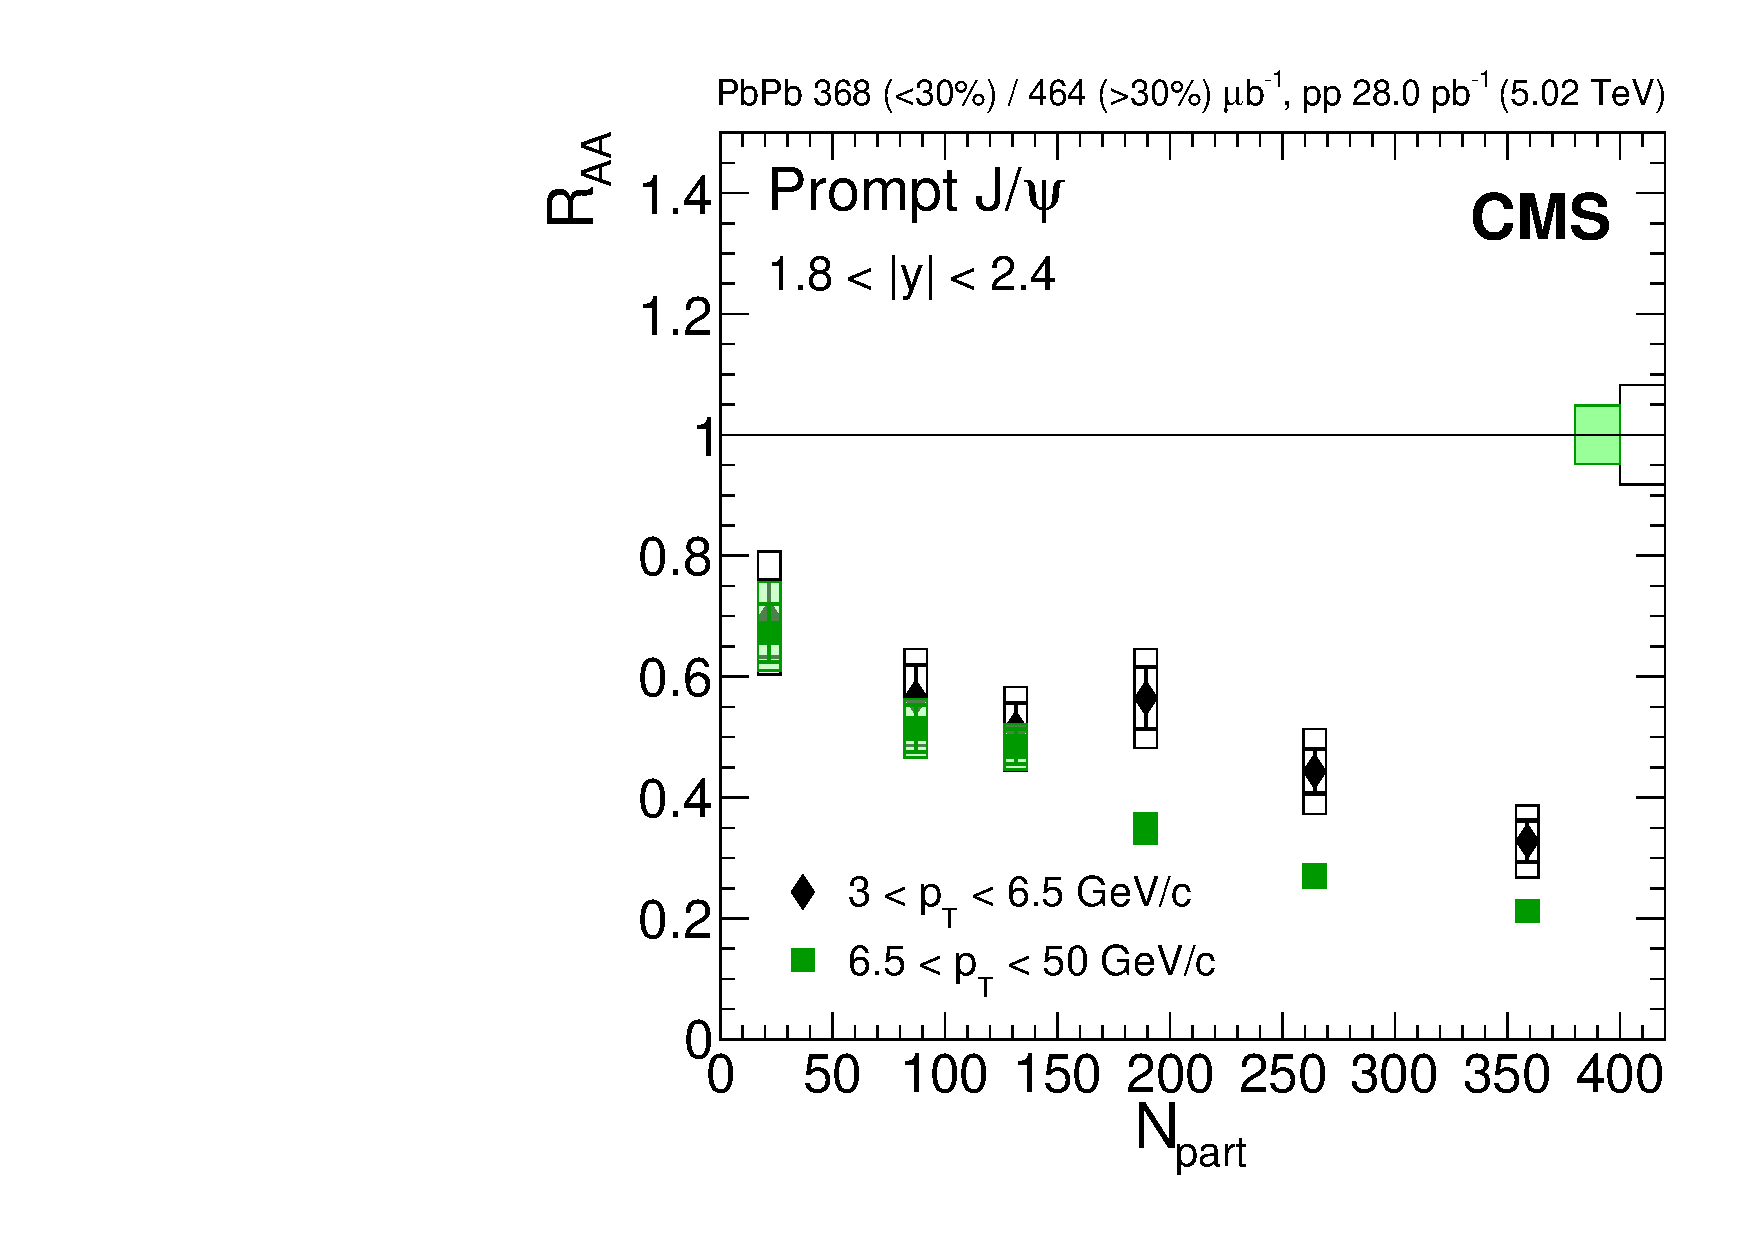
\includegraphics[width=0.45\textwidth]{Figures/Charmonia/Results/Prompt_JPsi_RAA/Figure_006-b.pdf}
 \caption{Nuclear modification factor of prompt \JPsi mesons. Left: as a function of \ptMuMu in the mid- and most forward rapidity regions. Right: as a function of \avgnpart at $3 < \ptMuMu < 6.5$~\GeVc and $6.5 < \ptMuMu < 50$~\GeVc, in the $1.8 < |\rapMuMu| < 2.4$ rapidity region. The boxes (bars) represent the systematic (statistical) uncertainties. The size of the global relative uncertainties are depicted in the boxes plotted at $\raa=1$. Figures published in Ref.~\cite{CMS_JPsi_PbPb_5p02TeV}.}
  \label{fig:PromptJpsi_RAA}
\end{figure}


\subsubsection{Nonprompt \texorpdfstring{\JPsi}{J/psi}-meson \texorpdfstring{\raa}{RAA}}\label{sec:Charmonia_Results_RAA_JPsi_Nonprompt}

The suppression of b hadrons is probed by the nuclear modification factor of nonprompt \JPsi mesons. The nonprompt \JPsi-meson results as a function of \pt, rapidity and \avgnpart are compared to the corresponding ones obtained at $\sqrtsnn = \SI{2.76}{\TeV}$ in \fig{fig:NonpromptJpsi_ComparisonWith2p76_RAA}. The measurements at both collision energies are also found to be in good overall agreement. 

\begin{figure}[htb!]
  \centering
    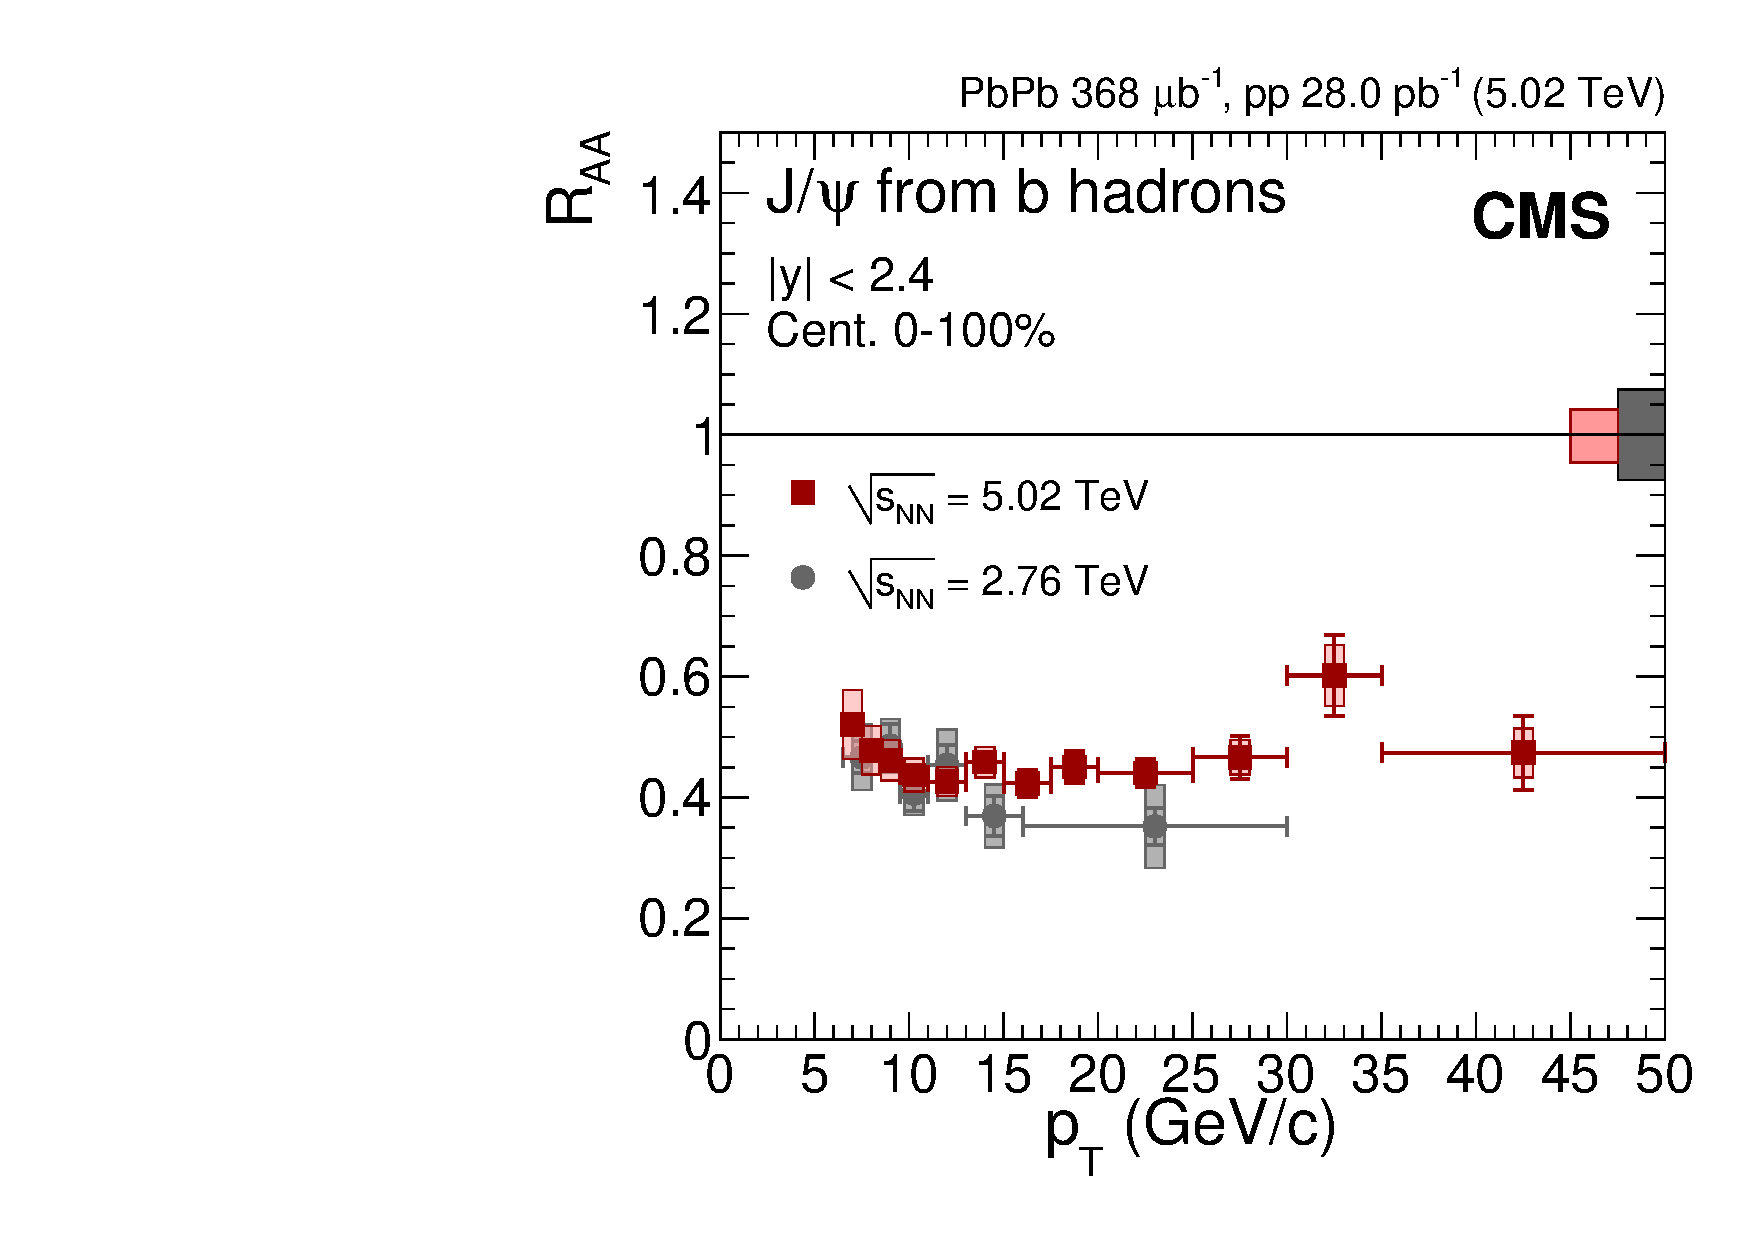
\includegraphics[width=0.32\textwidth]{Figures/Charmonia/Results/ComparisonWith2p76TeV/NonPrompt_JPsi_RAA/Figure_008-c.pdf}
    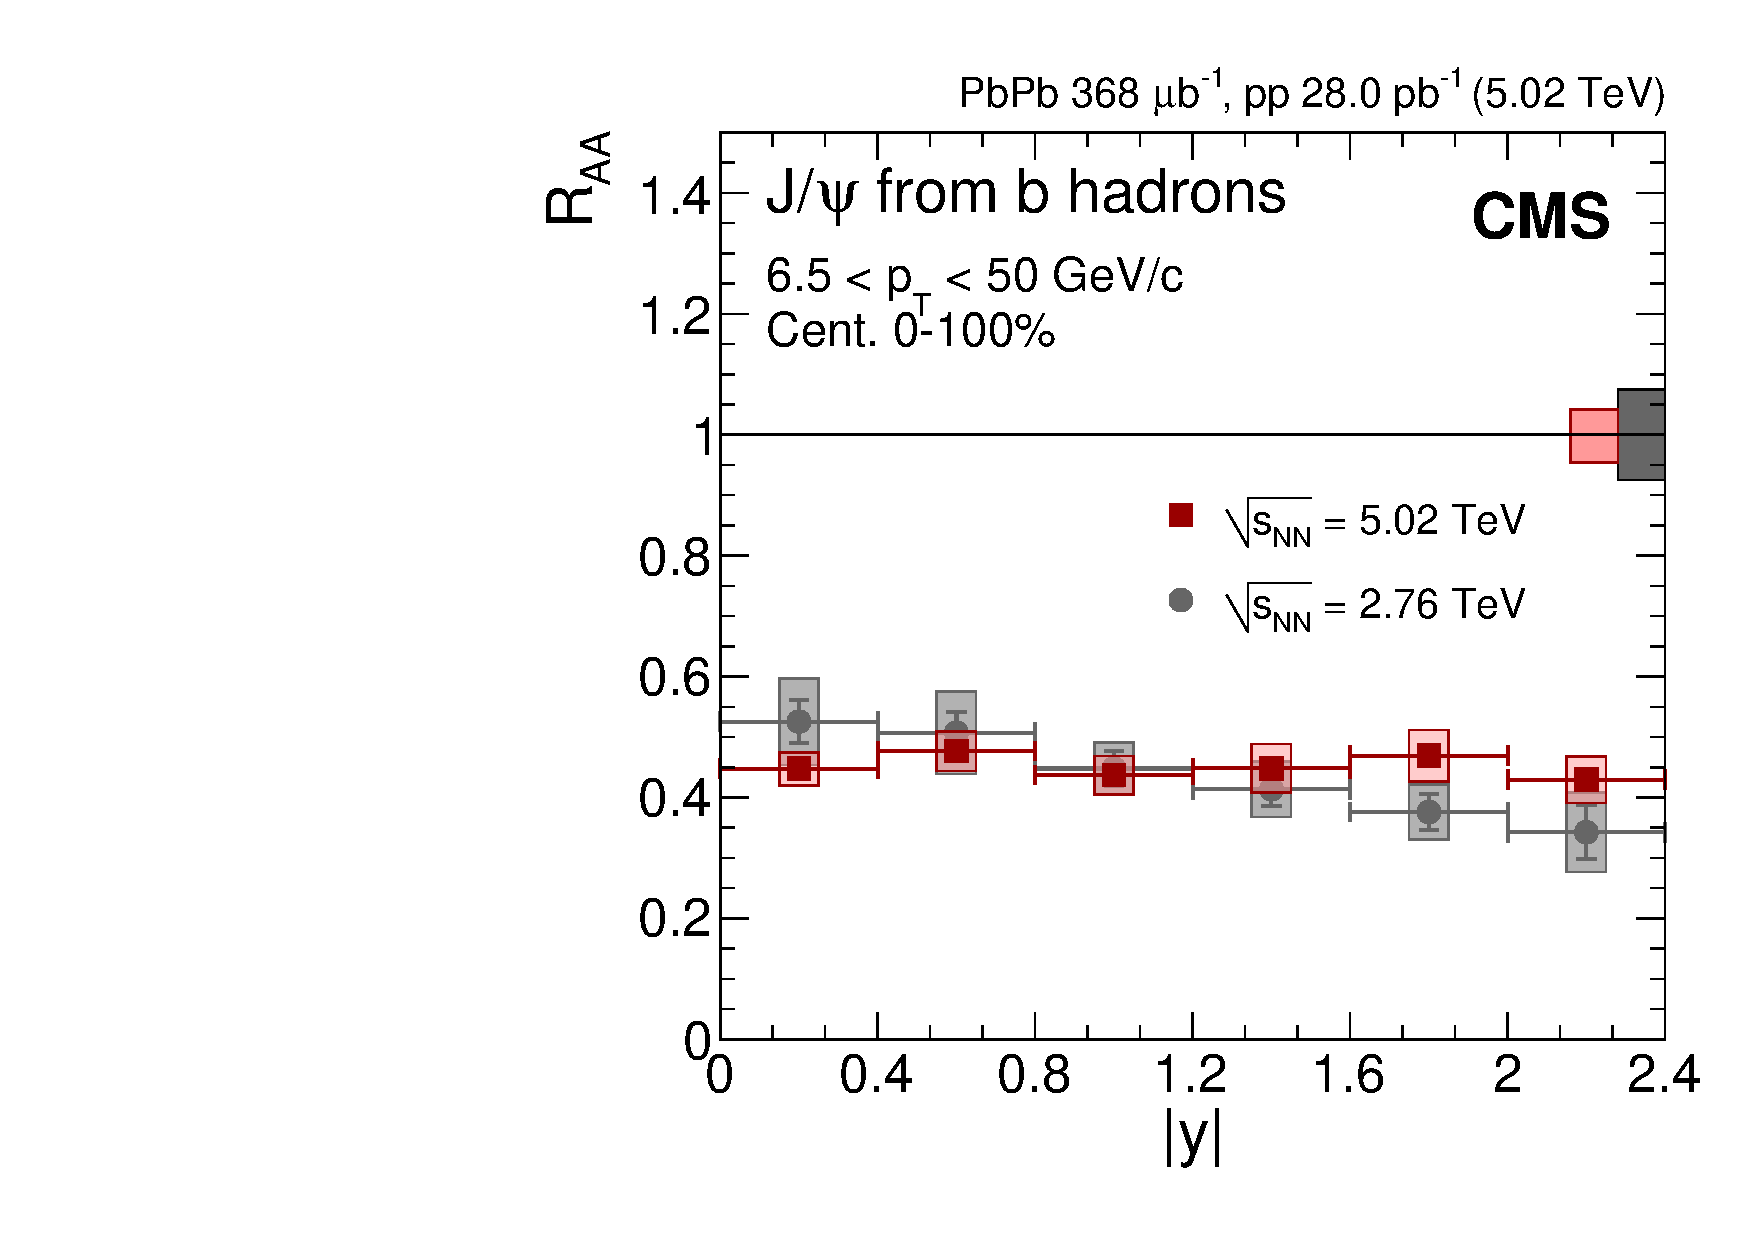
\includegraphics[width=0.32\textwidth]{Figures/Charmonia/Results/ComparisonWith2p76TeV/NonPrompt_JPsi_RAA/Figure_008-a.pdf}
    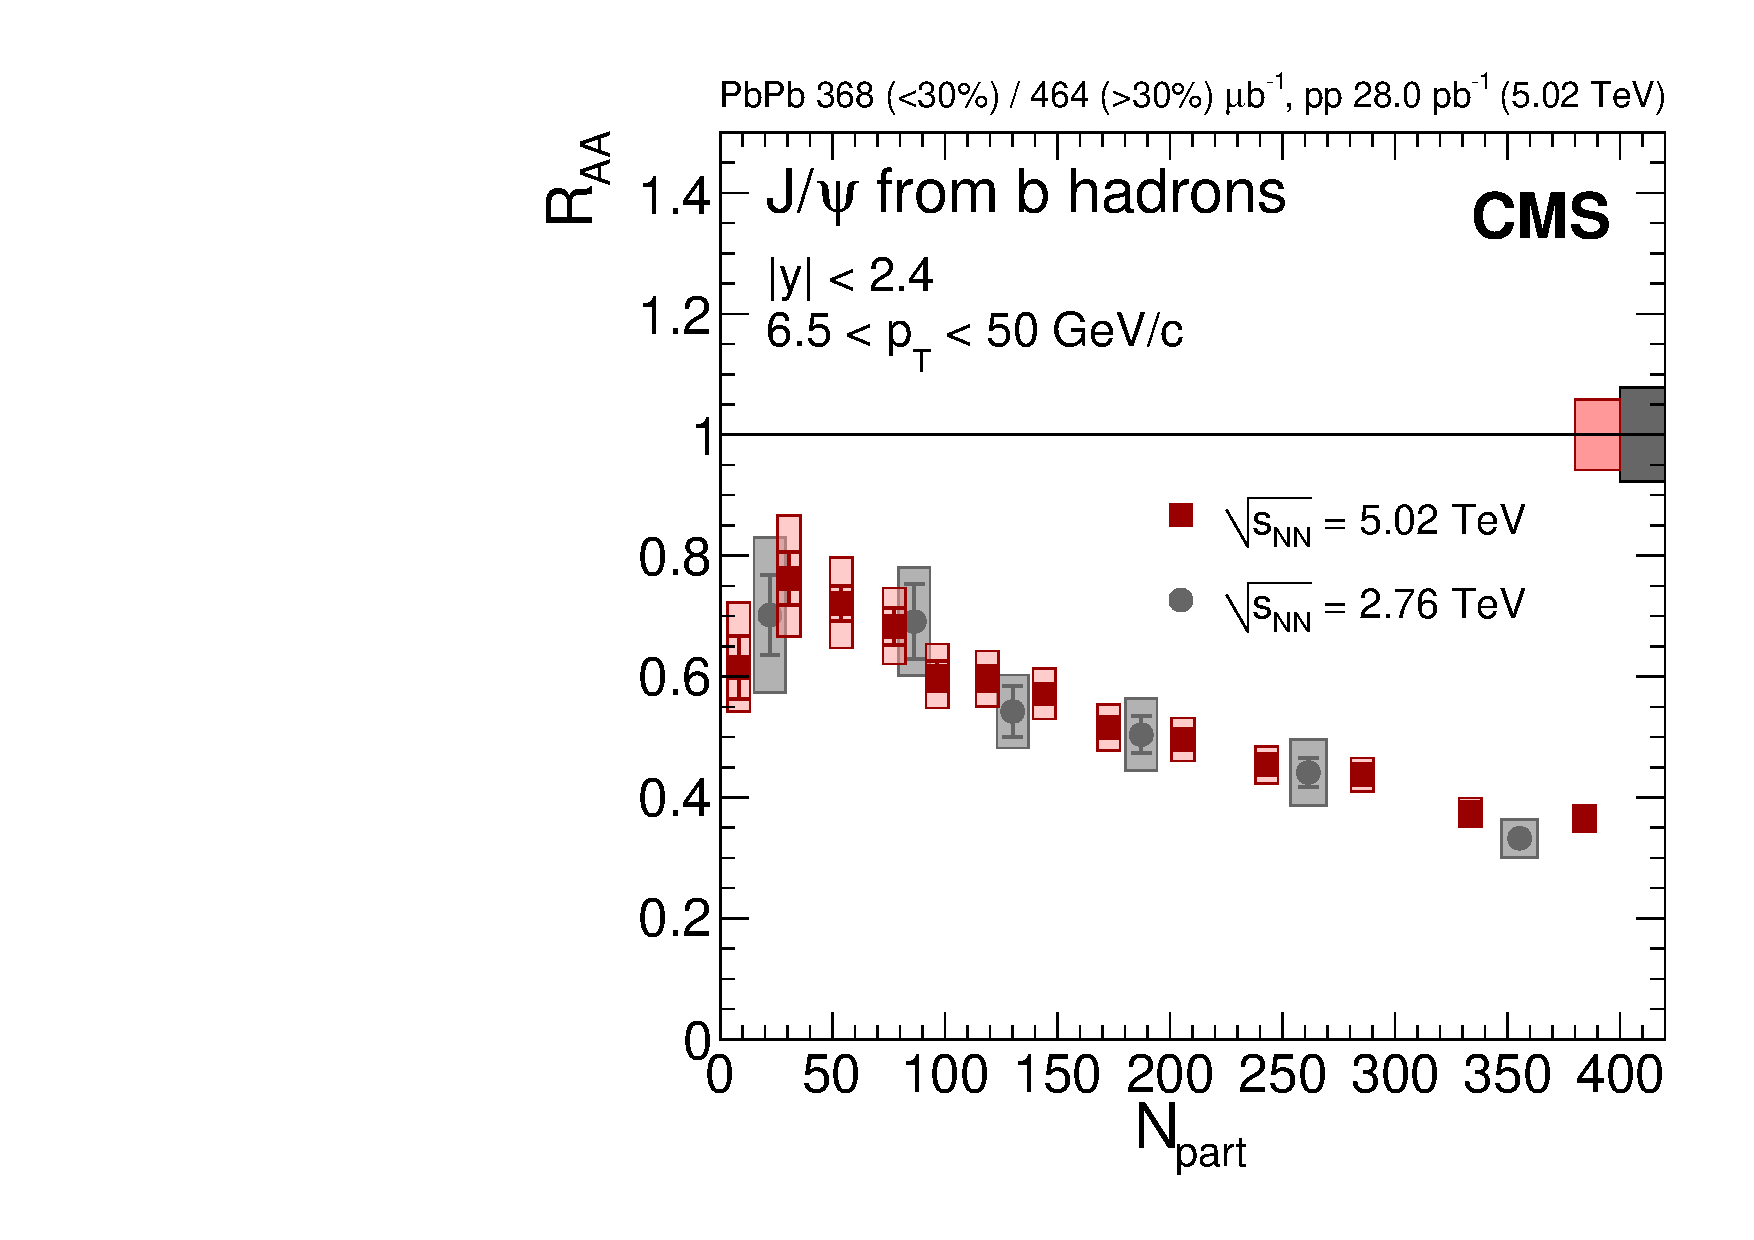
\includegraphics[width=0.32\textwidth]{Figures/Charmonia/Results/ComparisonWith2p76TeV/NonPrompt_JPsi_RAA/Figure_008-b.pdf}
    \caption{Nuclear modification factor of nonprompt \JPsi mesons measured at $\sqrtsnn = \SI{2.76}{\TeV}$~\cite{CMS_JPsi_PbPb_2p76TeV} (grey circles) and $\sqrtsnn = \SI{5.02}{\TeV}$~\cite{CMS_JPsi_PbPb_5p02TeV} (red squares), as a function of dimuon \pt (left), rapidity (middle) and \avgnpart (right). The boxes (bars) represent the systematic (statistical) uncertainties. The size of the global relative uncertainties are depicted in the boxes plotted at $\raa=1$. Figures published in Ref.~\cite{CMS_JPsi_PbPb_5p02TeV}.}
    \label{fig:NonpromptJpsi_ComparisonWith2p76_RAA}
\end{figure}

The b hadrons are suppressed in all measurements and the nonprompt \JPsi-meson \raa decreases towards high \ptMuMu reaching a value of $\raa \approx 0.4$. The suppression is observed to not vary significantly with respect to rapidity. In addition, the suppression of b hadrons becomes stronger for more central collisions. The nonprompt \JPsi-meson nuclear modification factor varies from $\raa \approx 0.7$ in the most peripheral centrality bin ($50-100\%$) to $\raa \approx 0.4$ for the most central \RunPbPb collisions ($0-10\%$).

In \fig{fig:NonpromptJpsi_RAA_pT}, the \raa of nonprompt \JPsi mesons is presented as a function of \ptMuMu in the mid- and forward rapidity regions (left), and \avgnpart in two \ptMuMu intervals (right). A hint of stronger suppression is seen in the highest \pt interval ($6.5 < \ptMuMu < 50$~\GeVc) as a function of \avgnpart, which could originate from parton energy loss (i.e. jet quenching) of bottom quarks in the QGP medium as detailed in \sect{sec:Physics_HI_Probes_JetQuenching}. More differential studies can be found in Ref.~\cite{CMS_JPsi_PbPb_5p02TeV}.

\begin{figure}[htb!]
 \centering
  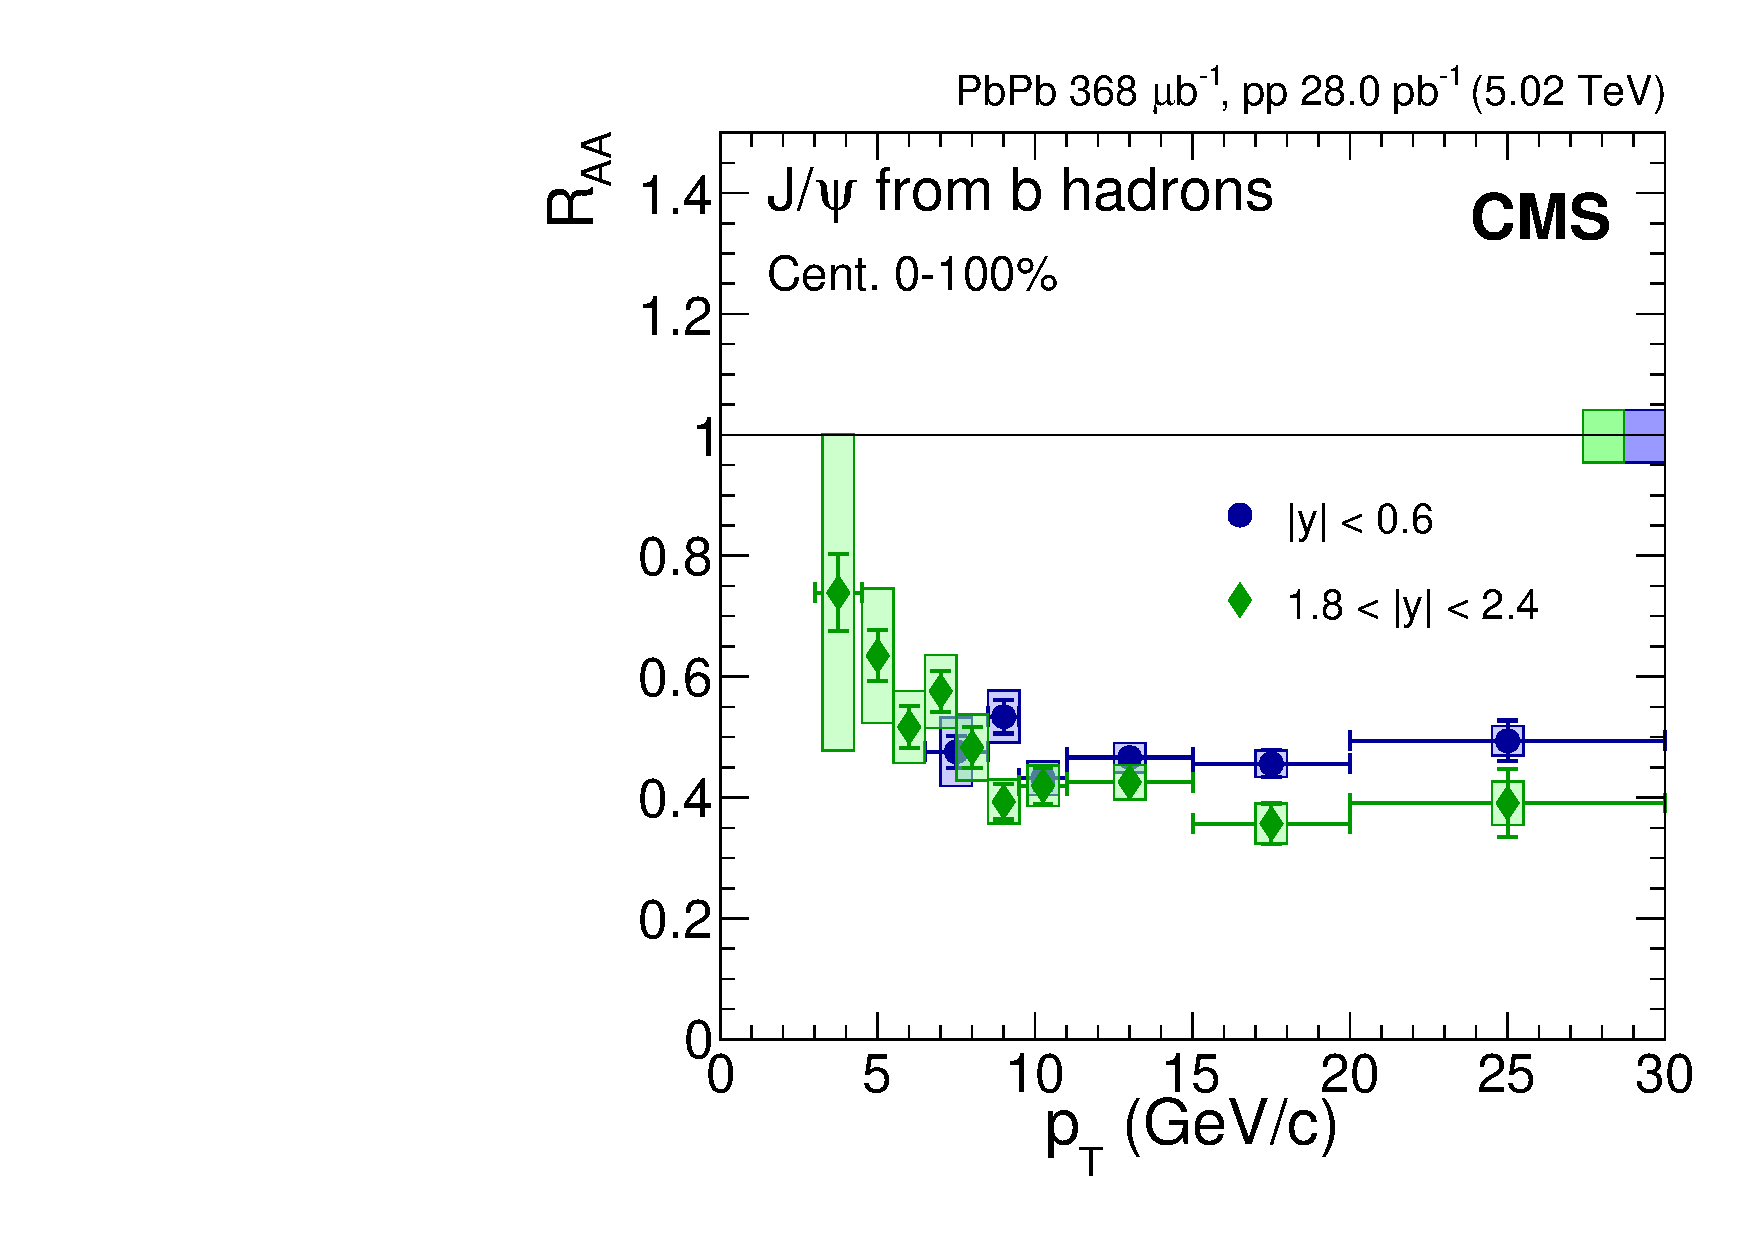
\includegraphics[width=0.45\textwidth]{Figures/Charmonia/Results/NonPrompt_JPsi_RAA/Figure_009-a.pdf}
  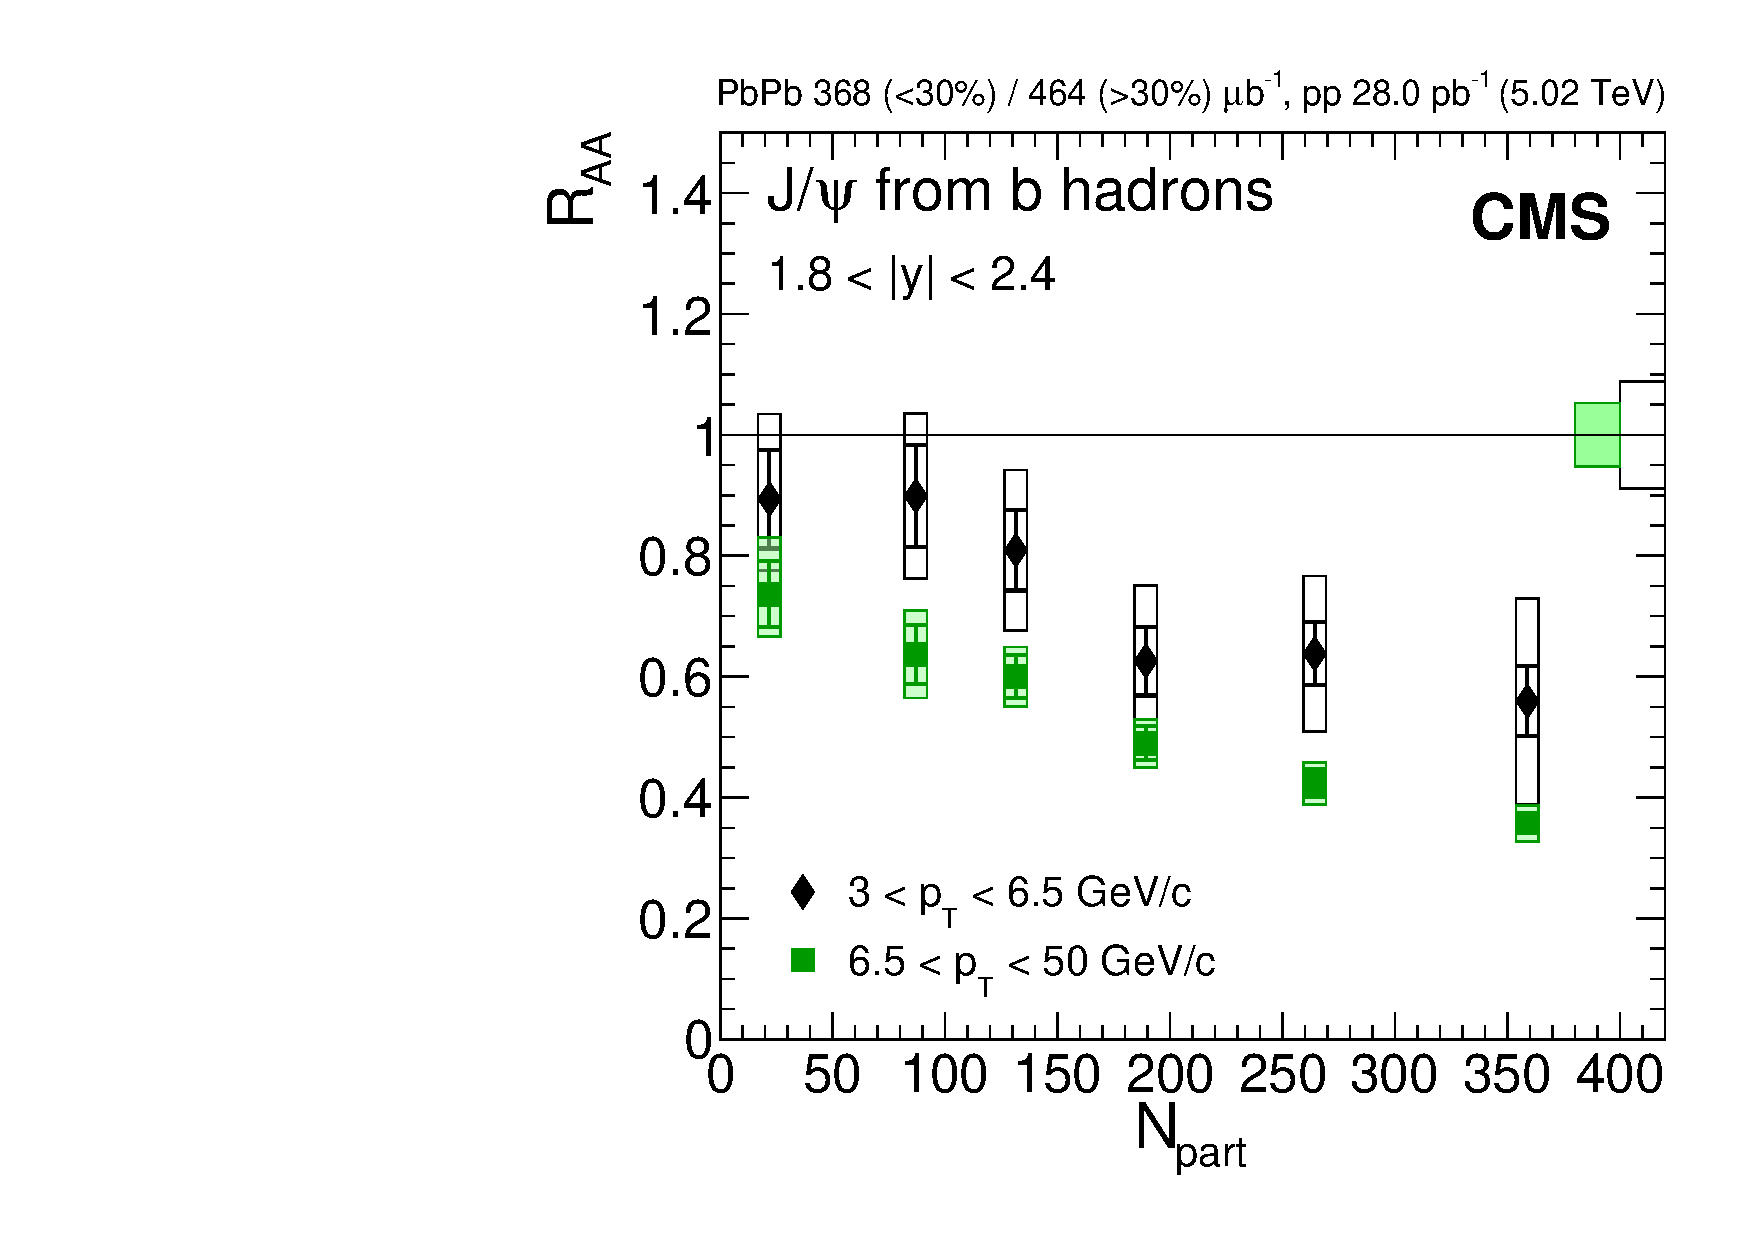
\includegraphics[width=0.45\textwidth]{Figures/Charmonia/Results/NonPrompt_JPsi_RAA/Figure_010-b.pdf}
  \caption{Nuclear modification factor of nonprompt \JPsi mesons. Left: as a function of \ptMuMu in the mid- and most forward rapidity regions. Right: as a function of \avgnpart in two \ptMuMu intervals at forward rapidity. The boxes (bars) represent the systematic (statistical) uncertainties. The size of the global relative uncertainties are depicted in the boxes plotted at $\raa=1$. Figures published in Ref.~\cite{CMS_JPsi_PbPb_5p02TeV}.}
  \label{fig:NonpromptJpsi_RAA_pT}
\end{figure}


\subsection{Double ratio of prompt \texorpdfstring{\PsiP}{psi(2S)}/\texorpdfstring{\JPsi}{J/psi} yields}\label{sec:Charmonia_Results_DoubleRatio}

The double ratio of prompt \PsiP over \JPsi meson yields, \doubleRatio, is derived from the \PsiP-to-\JPsi yields ratios measured in \Runpp and \RunPbPb collisions, as detailed in \sect{sec:Charmonia_Analysis_PsiPoverJPsiRatioExtraction}. The systematic uncertainties that affects the measurement of the double ratio of prompt charmonium yields are:
\begin{itemize}
 \item The uncertainty on the extraction of the \PsiP-to-\JPsi yields ratios, derived from the parametrisation of the \mMuMu distribution in \Runpp and \RunPbPb collisions. This uncertainty is found to be less than 0.02 (0.11) from the \Runpp (\RunPbPb) data fits.
 \item The uncertainty on the cancellation of the prompt charmonium efficiencies. This uncertainty is seen to vary between 0.01 and 0.05, except at $3 < \ptMuMu < 6.5$~\GeVc, where it seen to be 0.10.
 \item The uncertainty on the subtraction of the nonprompt charmonium contamination, which is less than 0.07.
\end{itemize}

The results of the \doubleRatio, as a function of \ptMuMu, are presented in \fig{fig:PromptCharmonium_DoubleRatio}. Since the values of the double ratios of prompt charmonium yields  and the prompt \JPsi-meson \raa are below unity in all measurements, the prompt \PsiP mesons are more suppressed than the prompt \JPsi mesons in \RunPbPb collisions. This is consistent with a sequential suppression of charmonia in the QGP. The results at mid- and forward rapidity regions are compatible within uncertainties, and no significant dependence is seen as a function of \ptMuMu.

\begin{figure}[!htb]
 \centering
  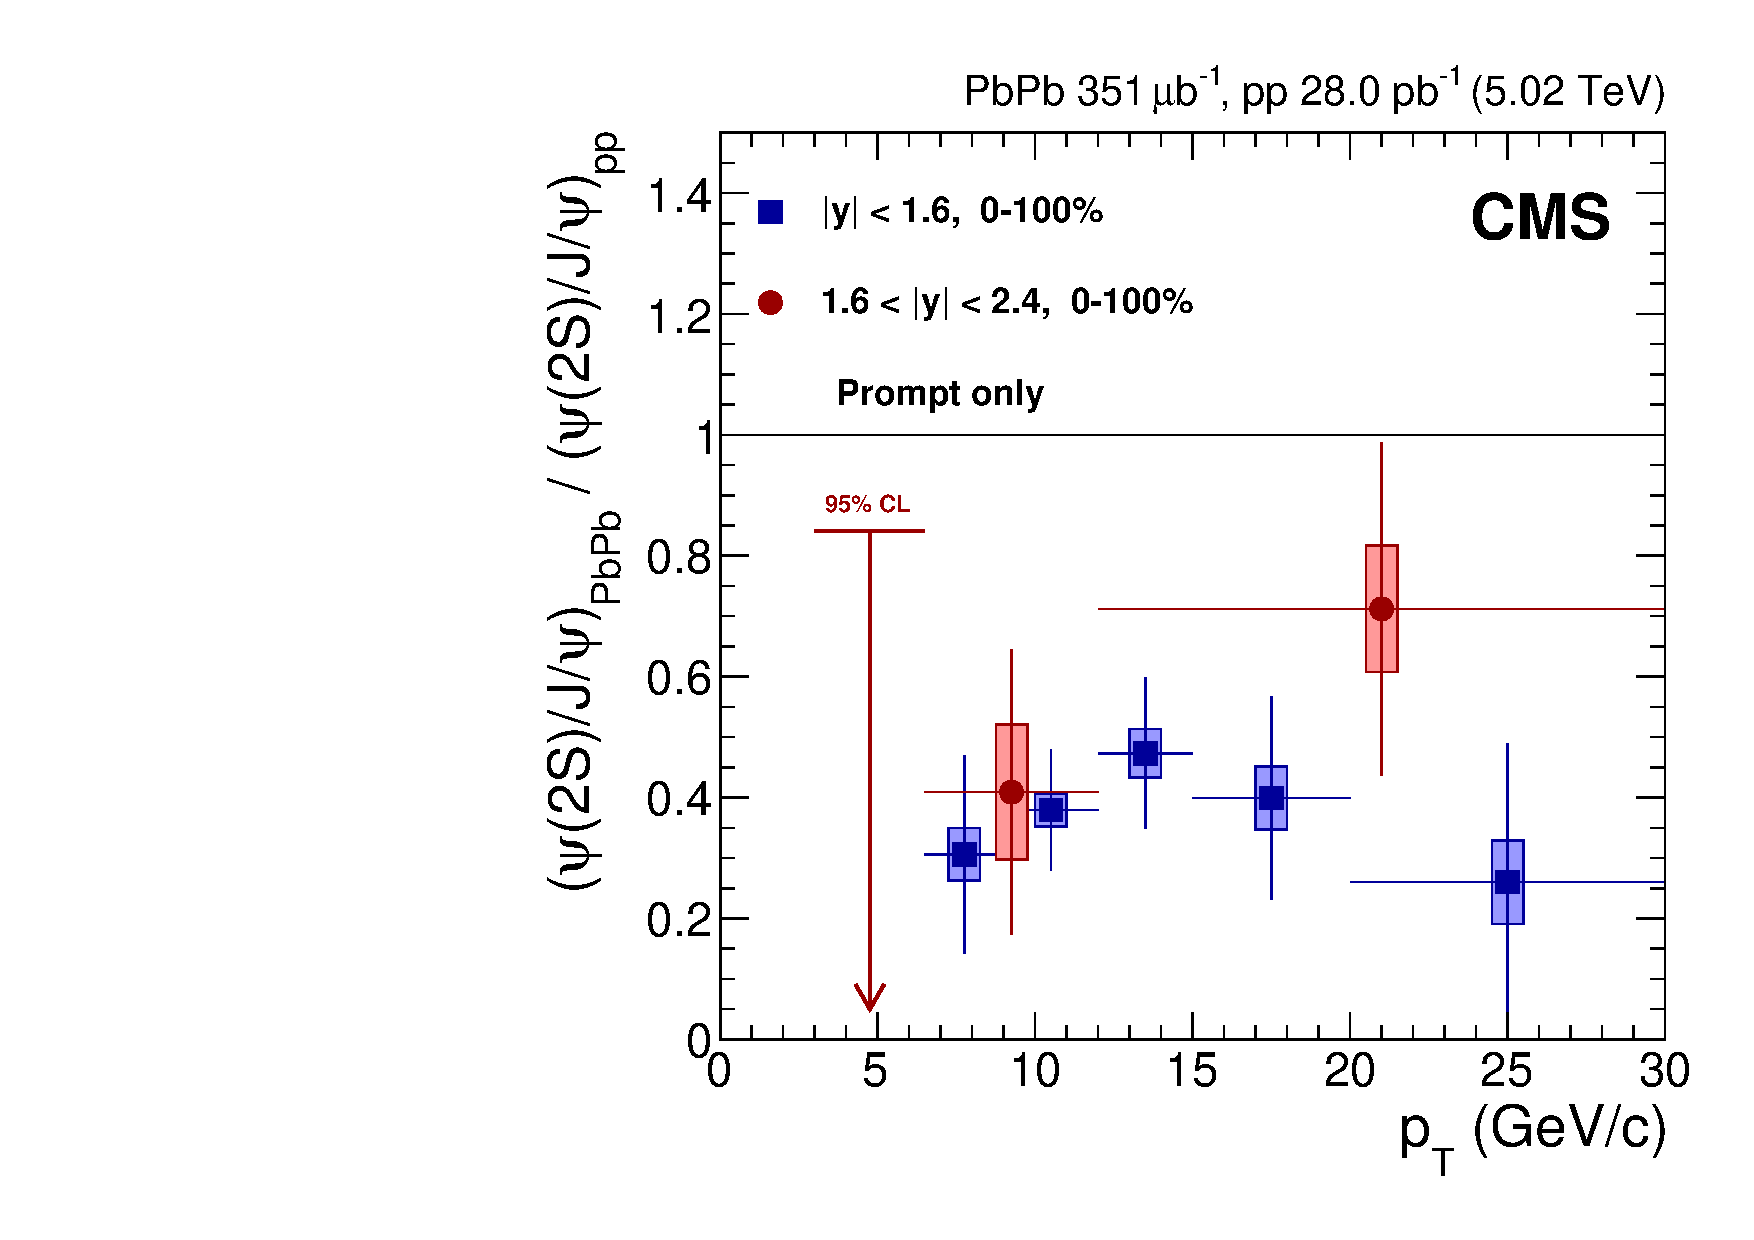
\includegraphics[width=0.48\textwidth]{Figures/Charmonia/Results/Prompt_Charmonium_DoubleRatio/Figure_002.pdf}
 \caption{Double ratio of prompt \PsiP over \JPsi meson yields as a function of the dimuon \pt, at $|\rapMuMu| < 1.6$ (squares) and $1.6 < |\rapMuMu| < 2.4$ (circles). The horizontal lines denotes the widths of the \pt intervals. The bars (boxes) represent the statistical (systematic) uncertainties, while the arrows indicate the 95\% CL interval where the measurement is consistent with zero. Figures published in Ref.~\cite{CMS_Psi2S_PbPb_5p02TeV}.}
 \label{fig:PromptCharmonium_DoubleRatio}
\end{figure}

The measurements of the double ratio of prompt charmonium yields are also performed for different centrality intervals, as shown in terms of \avgnpart in \fig{fig:PromptCharmonium_ComparisonWith2p76_DoubleRatio}, separately for mid-rapidity (left) and forward rapidity (right). The results do not exhibit a clear dependence with respect to \avgnpart. Moreover, the  double ratios measured in the $20-100\%$ centrality range at forward rapidity and the most central collisions ($0-20\%$) at mid-rapidity, are consistent with zero. The results at $\sqrtsnn = \SI{5.02}{\TeV}$ are compared with the previous CMS measurement at $\sqrtsnn = \SI{2.76}{\TeV}$. On the one hand, the results with respect to \avgnpart at both energies are observed to be compatible in the mid-rapidity region at $6.5 < \ptMuMu < 30$~\GeVc. On the other hand, the measurements extending to lower \ptMuMu intervals ($3 < \ptMuMu < 30$) in the forward rapidity region are strongly reduced at $\sqrtsnn = \SI{5.02}{\TeV}$ compared to $\sqrtsnn = \SI{2.76}{\TeV}$, and the enhancement present at $\sqrtsnn = \SI{2.76}{\TeV}$ for the most central collisions is not seen at $\sqrtsnn = \SI{5.02}{\TeV}$. The difference in the centrality-integrated interval, between $\sqrtsnn = \SI{2.76}{\TeV}$ and $\sqrtsnn = \SI{5.02}{\TeV}$, corresponds to roughly 3 standard deviations.

\begin{figure}[htb!]
 \centering
  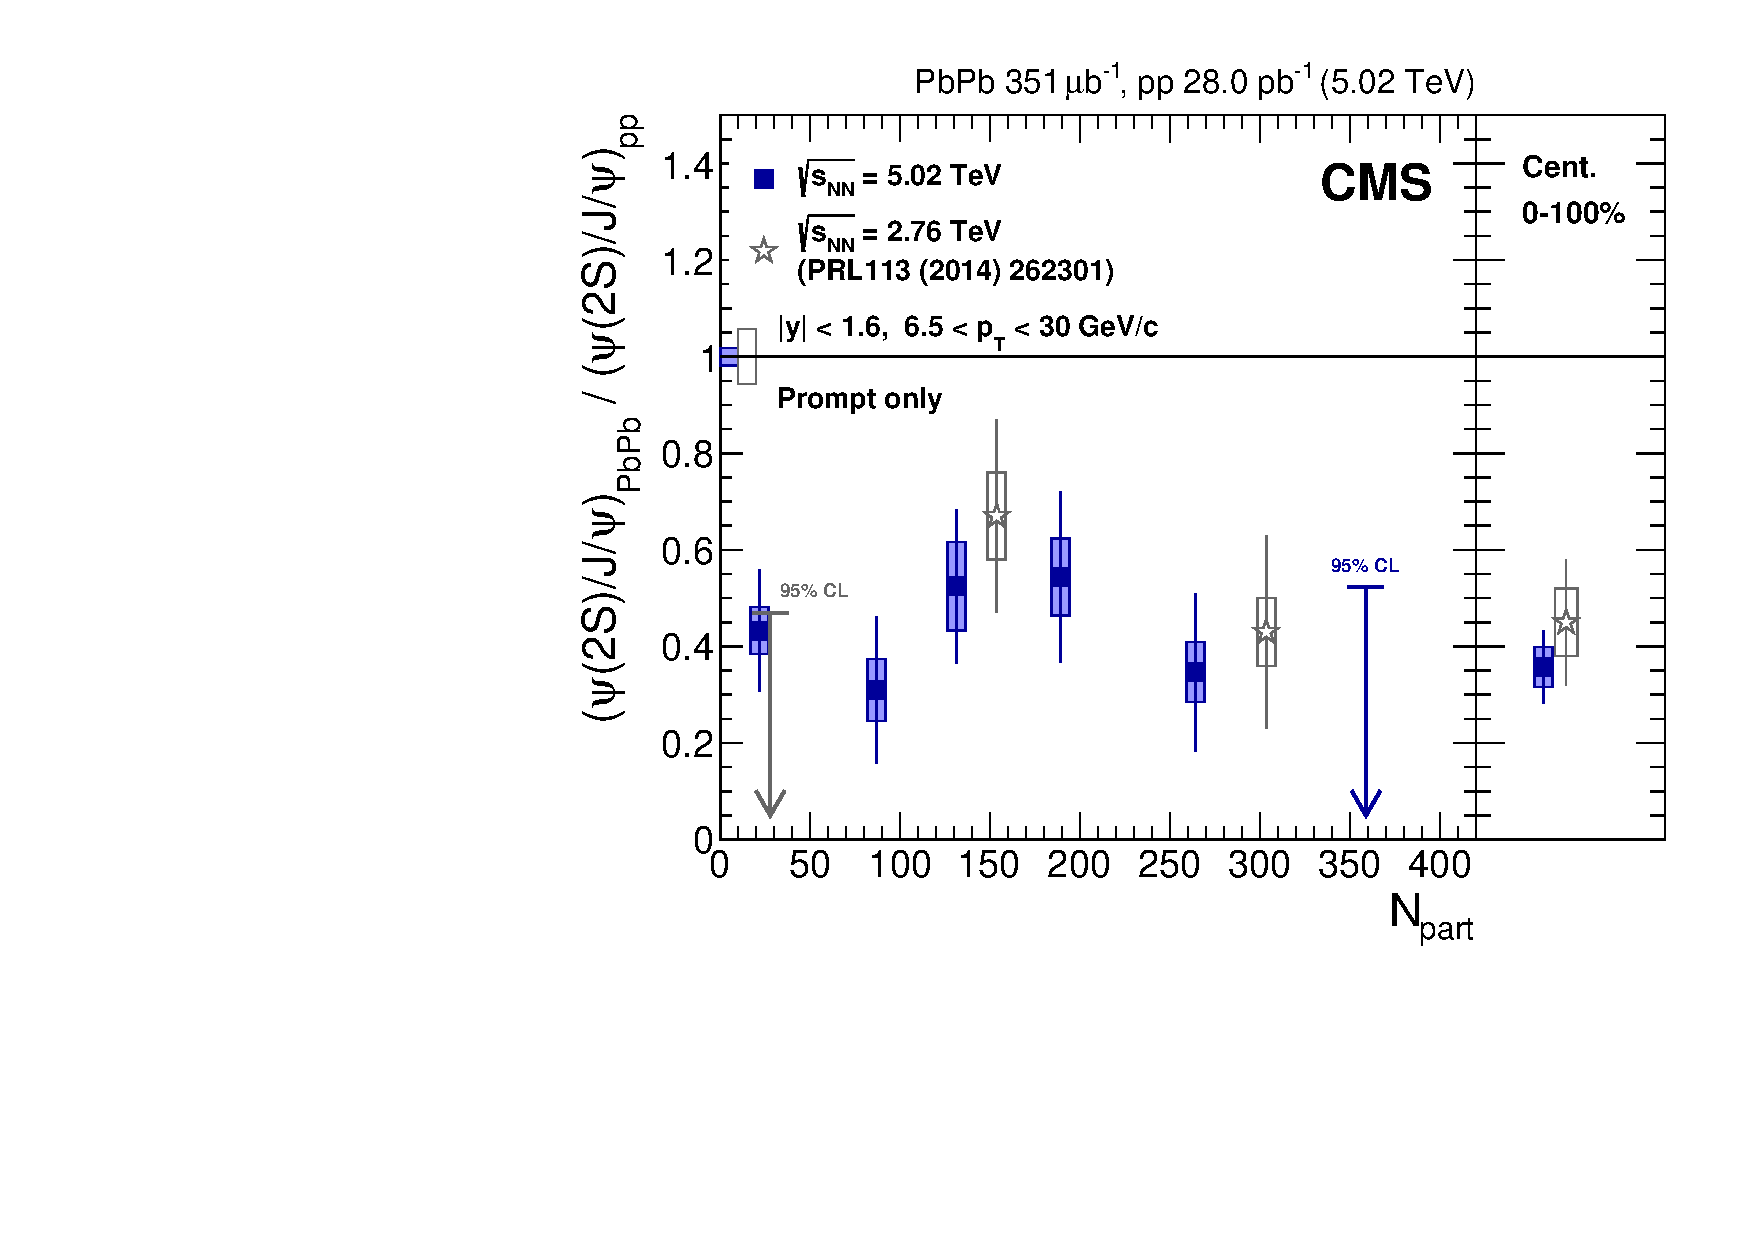
\includegraphics[width=0.45\textwidth]{Figures/Charmonia/Results/ComparisonWith2p76TeV/Prompt_Charmonium_DoubleRatio/Figure_003-a.pdf}
  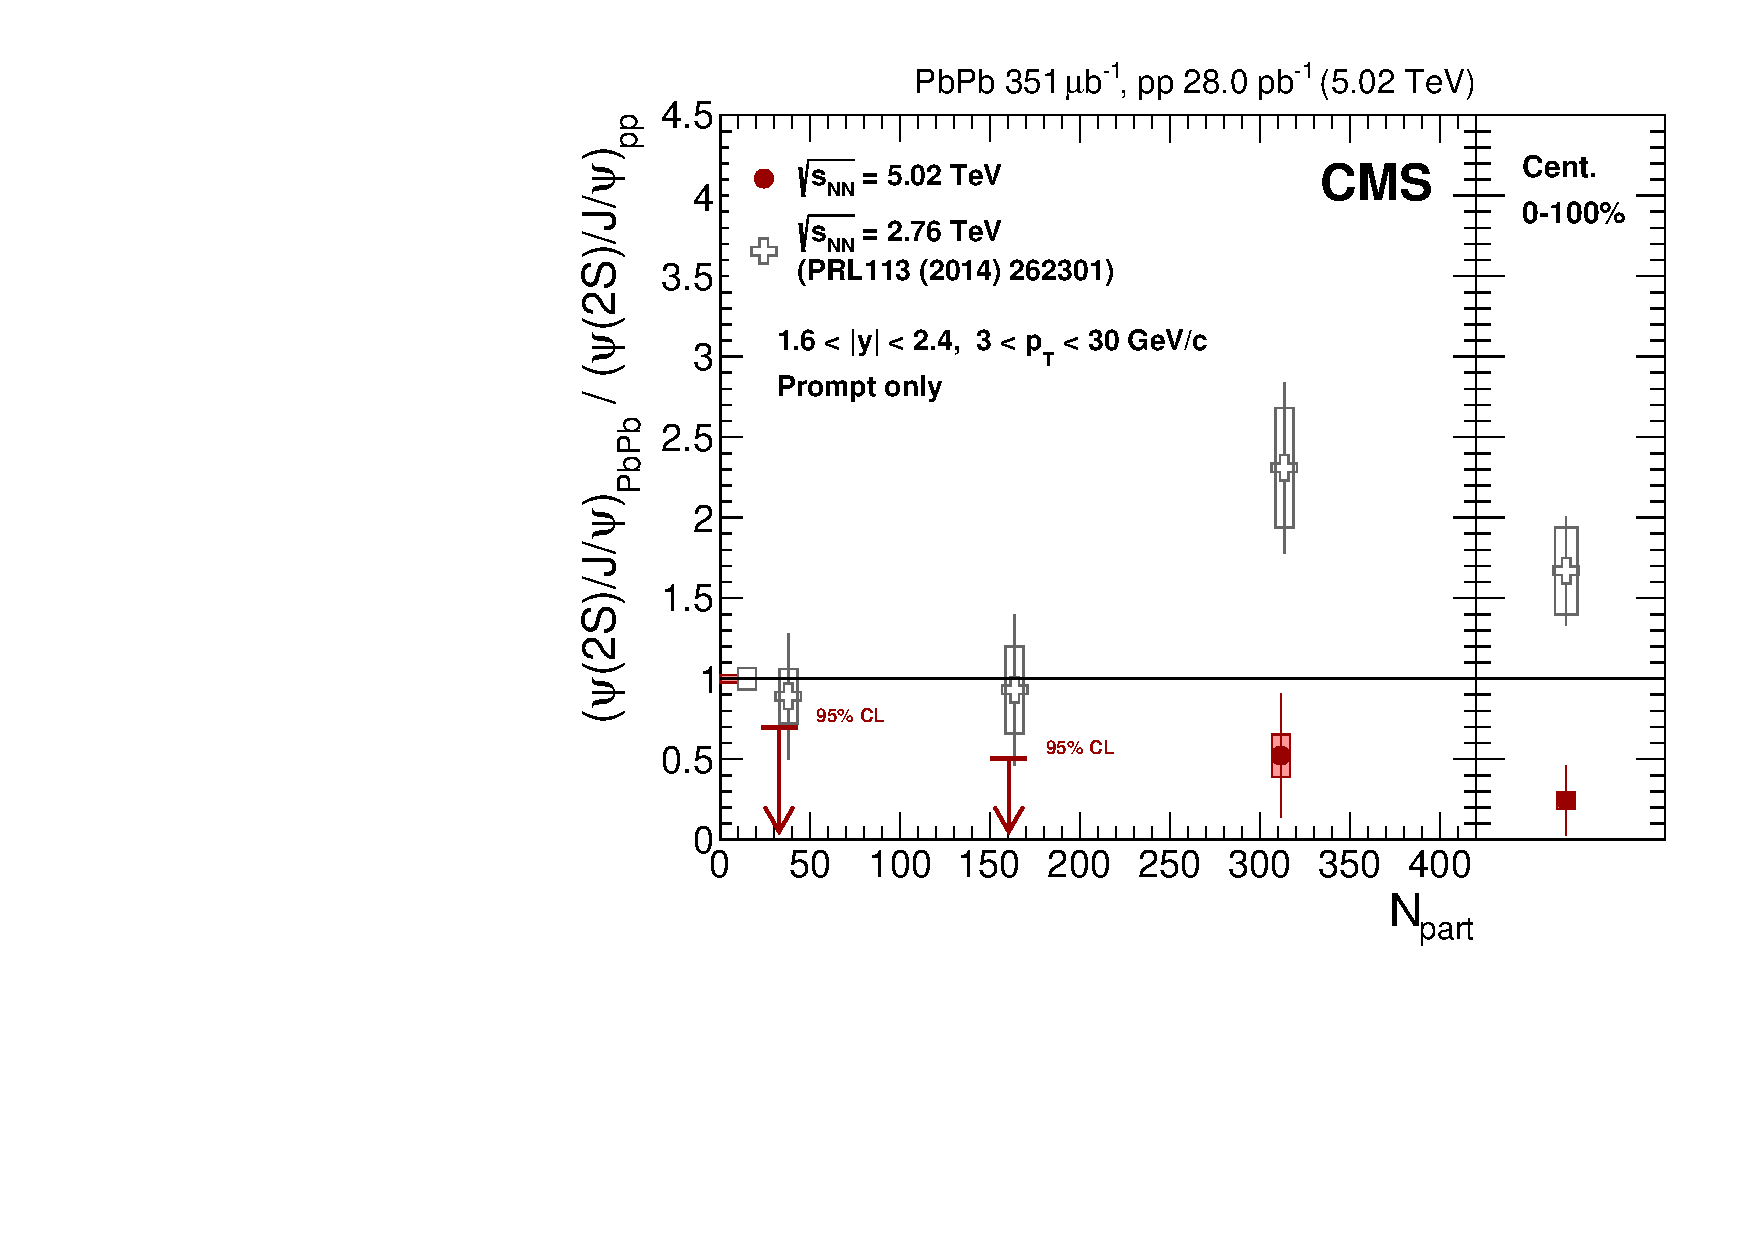
\includegraphics[width=0.45\textwidth]{Figures/Charmonia/Results/ComparisonWith2p76TeV/Prompt_Charmonium_DoubleRatio/Figure_003-b.pdf}
 \caption{Comparison of the double ratio of prompt \PsiP over \JPsi meson yields measured at $\sqrtsnn = \SI{2.76}{\TeV}$~\cite{CMS_Psi2S_PbPb_2p76TeV} and $\sqrtsnn = \SI{5.02}{\TeV}$~\cite{CMS_Psi2S_PbPb_5p02TeV}, as a function of the dimuon \pt (left) and \RunPbPb collision centrality (right), at $|\rapMuMu| < 1.6$ (squares) and $1.6 < |\rapMuMu| < 2.4$ (circles). The horizontal lines denotes the widths of the \pt intervals. The bars (boxes) represent the statistical (systematic) uncertainties, while the arrows indicate the 95\% CL interval where the measurement is consistent with zero. Figures published in Ref.~\cite{CMS_Psi2S_PbPb_5p02TeV}.}
 \label{fig:PromptCharmonium_ComparisonWith2p76_DoubleRatio}
\end{figure}

A possible interpretation of the double ratio results is provided by Ralf Rapp and Xiaojian Du in Ref.~\cite{DoubleRatioTheory_2}, using a transport model approach. According to Rapp and Du, the enhancement observed at $\sqrtsnn = \SI{2.76}{\TeV}$ could be a signature of sequential regeneration of charmonia. They propose that \PsiP mesons are regenerated later in the medium evolution, where the larger collective flow shifts their transverse momentum to $\pt > 3$~\GeVc, while the \JPsi mesons are mainly regenerated earlier at lower \pt~\cite{DoubleRatioTheory}. However, at higher collisions energies, the \pt spectrum of the regenerated \JPsi mesons is shifted to $\pt > 3$~\GeVc due to the increase in transverse flow, leading to the suppression pattern observed at $\sqrtsnn = \SI{5.02}{\TeV}$.

% END OF SECTION